\chapter{度量空间}
\label{chap:metric-spaces}

用迭代$x^{(t+1)}=x^{(t)}/2+1$求解方程$x=x/2+1$时，相邻两次结果的差每步减半，我们很快会相信迭代“收敛”。但这份信心需要回答两个问题：误差为什么会趋于零，以及点列逼近的那个极限是否真的存在于我们允许取值的范围内。在有理数中用$1,\ 1.4,\ 1.41,\ 1.414,\dots$逼近$\sqrt2$时，相邻项同样越来越近，极限却不在有理数中。可见“越来越近”与“有极限”是两件事，后者还取决于空间本身。

同样的问题出现在实数和向量以外的对象上。比较两段等长的二进制串、图中的两个顶点或两种特征表示时，对象不能相减，但我们仍要说它们相距多远、一列对象是否趋于某个对象、一个映射会不会把小的输入差异放大成大的输出差异。本章的学习目标，是从距离的几条共同规则出发，建立一套不依赖坐标的邻近、收敛与连续语言，并弄清每个结论所需的条件。

路线由这些问题的依赖关系决定。先规定什么样的规则可以称为距离，以及怎样由已有距离构造新距离；距离给定后，才能谈一点附近有哪些点、集合是否包含它的邻近点。点列收敛把邻近关系变成可以逐项检查的误差，完备性回答极限是否留在空间中，紧致性则用有限个小球控制整个集合，从而保证收敛子列和极值存在。连续映射研究误差怎样在两个空间之间传递，空间之间的比较说明哪些性质能经由映射保留。最后，这些工具在压缩映射定理中汇合：误差几何地缩小，点列是柯西列，完备性给出极限，连续性验证它是方程的解。

\section{度量与度量空间}
\label{sec:metric-definition}

实数之间用绝对值比较远近，向量之间用范数比较远近，二进制串之间可以数有多少位不同，图中两个顶点之间可以数最少要走几条边。这些比较方法的对象和计算方式各不相同，却共同遵守几条规则。本节先把这些规则提炼为度量的定义，再列出常见度量，最后研究在只看一部分对象、组合多个对象或忽略部分差异时，怎样从已有度量得到新的度量。

\subsection{度量的定义}
\label{sec:metric-axioms}

在实轴上，$|x-y|$不取负值，只在$x=y$时为零，与两数的先后无关，并且满足$|x-z|\leq|x-y|+|y-z|$。平面上的欧氏距离也具有这四条性质。后面关于邻近、收敛和连续的论证只用到这四条性质，因此把它们取为定义。

\begin{definition}[度量与度量空间]
\label{def:metric-space}
设$X$是非空集合。若函数$d:X\times X\to[0,\infty)$对任意$x,y,z\in X$满足
\begin{enumerate}
  \item 分离性：$d(x,y)=0$当且仅当$x=y$；
  \item 对称性：$d(x,y)=d(y,x)$；
  \item 三角不等式：$d(x,z)\leq d(x,y)+d(y,z)$，
\end{enumerate}
就称$d$为$X$上的一个\term{度量}（metric），也称距离函数；称$(X,d)$为\term{度量空间}（metric space），$d(x,y)$称为$x$与$y$之间的距离。
\end{definition}

陪域取为$[0,\infty)$已经包含了非负性，并且要求距离总是有限的实数。这四条要求各自排除一种不合适的比较方式。非负性排除了“负的远近”；分离性要求不同的点距离严格为正，比较规则能够辨认不同对象；对称性要求从$x$看$y$与从$y$看$x$得到同一个数。三角不等式最为关键：经过中间点$y$绕行的总长度，不会短于直接从$x$到$z$的距离。正因为如此，一段难以直接估计的距离可以拆成几段容易估计的距离再相加。

\paragraph{反向三角不等式}
三角不等式给出距离之和的上界；后面的极限估计还常常需要两个距离之差的上界。对任意$x,y,z\in X$，三角不等式给出$d(x,z)\leq d(x,y)+d(y,z)$，即$d(x,z)-d(y,z)\leq d(x,y)$；交换$x$与$y$的角色，又得到$d(y,z)-d(x,z)\leq d(x,y)$。两式合起来就是
\begin{equation}
\label{eq:metric-reverse-triangle}
  \bigl|d(x,z)-d(y,z)\bigr|\leq d(x,y).
\end{equation}
它说明：把比较点从$x$移动到$y$，到固定点$z$的距离至多改变$d(x,y)$。图~\ref{fig:metric-triangle}把两种不等式画在同一个三角形中。

\begin{figure}[!htbp]
  \centering
  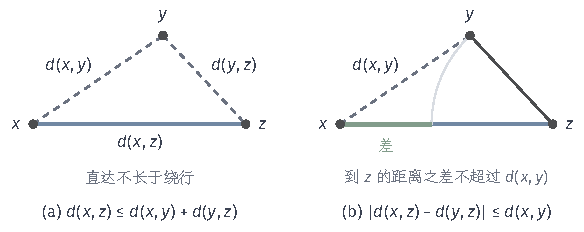
\includegraphics[width=98.972mm]{figures/02-abstract-mathematics/01-metric-and-measure/tikz/c1-triangle-inequality/figure.pdf}
  \caption{三角不等式与反向三角不等式。(a) 从$x$到$z$的直达距离（蓝色实线）不超过经中间点$y$的绕行长度（灰色虚线）。(b) 把比较点从$x$移到$y$时，到固定点$z$的两段距离之差（绿色标出的长度差）不超过移动的距离$d(x,y)$。}
  \label{fig:metric-triangle}
\end{figure}

\paragraph{集合与度量一起给出}
同一个集合可以配备不同的度量，所以度量空间是集合与度量组成的对，而不是集合本身。例如在$\mathbb R$上，除了通常距离$|x-y|$，还可以取下一小节的离散距离：任意两个不同的数距离都是$1$。在通常距离下，$1/n$与$0$的距离$1/n$越来越小；在离散距离下，这个距离始终是$1$。因此“$1/n$是否接近$0$”没有脱离度量的答案。后面凡是谈到邻近、收敛和连续，都要先说明使用的是哪个度量；在不致混淆时，才把$(X,d)$简称为$X$。

\subsection{常见度量}
\label{sec:metric-examples}

最常见的度量来自向量的范数；但度量并不要求对象能做减法，计数和路径长度同样可以给出度量。

\paragraph{由范数诱导的度量}
设$\lVert\cdot\rVert$是$\mathbb R^d$上的一个范数，即满足正定性、正齐次性$\lVert c\bm x\rVert=|c|\,\lVert\bm x\rVert$与三角不等式$\lVert\bm x+\bm y\rVert\leq\lVert\bm x\rVert+\lVert\bm y\rVert$的非负函数；常用的$\ell^1$、欧氏和最大值范数及其性质见\BookChapterRef{chap:normed-inner-product-spaces}{卷一“赋范空间与内积空间”章}。令$d(\bm x,\bm y)=\lVert\bm x-\bm y\rVert$，度量的三条要求逐条来自范数公理：正定性给出$d(\bm x,\bm y)=0\Leftrightarrow\bm x-\bm y=\bm 0$；取$c=-1$得到$\lVert\bm y-\bm x\rVert=\lVert\bm x-\bm y\rVert$，即对称性；把$\bm x-\bm z$写成$(\bm x-\bm y)+(\bm y-\bm z)$再用范数三角不等式，就得到度量的三角不等式。三种常用范数给出
\[
  \begin{aligned}
    d_1(\bm x,\bm y)&=\sum_{i=1}^d|x_i-y_i|,\qquad
    d_2(\bm x,\bm y)=\Bigl(\sum_{i=1}^d|x_i-y_i|^2\Bigr)^{1/2},\\
    d_\infty(\bm x,\bm y)&=\max_{1\leq i\leq d}|x_i-y_i|.
  \end{aligned}
\]
$d_1$把各坐标的偏差全部累加，$d_\infty$只记录最大的一个坐标偏差，$d_2$介于两者之间。

\begin{example}[同一组点的三种距离]
\label{ex:metric-three-distances}
在$\mathbb R^2$中取$\bm p=(0,0)$、$\bm q=(4,0)$、$\bm r=(3,3)$。$\bm q-\bm p=(4,0)$只有一个坐标偏差，三种距离都等于$4$。$\bm r-\bm p=(3,3)$的偏差分在两个坐标上，于是
\[
  d_1(\bm p,\bm r)=6,\qquad d_2(\bm p,\bm r)=3\sqrt2\approx4.243,\qquad d_\infty(\bm p,\bm r)=3.
\]
在$d_1$和$d_2$下$\bm q$离$\bm p$更近，在$d_\infty$下却是$\bm r$更近。图~\ref{fig:metric-three-distances}画出了三种读数：$d_1$沿坐标方向折线累加，$d_2$取直线段，$d_\infty$只看较长的那条坐标边。哪个点“更近”取决于我们怎样累计各坐标上的偏差。
\end{example}

\begin{figure}[!htbp]
  \centering
  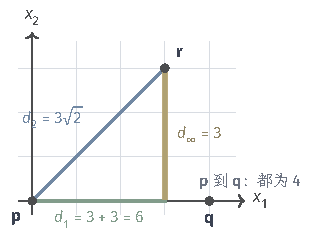
\includegraphics[width=52.871mm]{figures/02-abstract-mathematics/01-metric-and-measure/tikz/c1-three-distances/figure.pdf}
  \caption{同一组平面点在三种度量下的距离。$\bm q$与$\bm p$只在横坐标上相差$4$，三种距离都是$4$；$\bm r$与$\bm p$在两个坐标上各差$3$，$d_1$按折线累加得$6$，$d_2$取直线长度$3\sqrt2$，$d_\infty$只取较大的坐标差$3$。}
  \label{fig:metric-three-distances}
\end{figure}

\paragraph{不需要减法的度量}
在任意非空集合$X$上令$d(x,y)=0$（$x=y$）、$d(x,y)=1$（$x\neq y$），得到\term{离散度量}（discrete metric）。前两条要求直接由定义成立；对三角不等式，若$x=z$，左边为$0$；若$x\neq z$，则$y$不可能同时等于$x$和$z$，右边至少有一项为$1$。离散度量只回答“相同或不同”，不衡量差别大小，常用来构造反例。

对长度为$m$的两个二进制串$x=x_1\cdots x_m$与$y=y_1\cdots y_m$，\term{Hamming距离}（Hamming distance）定义为不同位置的个数$d_H(x,y)=\#\{i:x_i\neq y_i\}$，其中$\#$表示集合的元素个数。例如$d_H(10110,11100)=2$，两串在第2、4位不同。三角不等式逐位检查：若$x_i\neq z_i$，则$x_i\neq y_i$与$y_i\neq z_i$至少有一个成立，所以$x$与$z$不同的位置都被计入右边两项中的至少一项。这里用的是逐坐标比较，而不是对串做减法。

设$\mathcal G=(V,E)$是无权、无向的连通图，令$d_{\mathcal G}(u,v)$为从$u$到$v$的路径所含边数的最小值，即\term{最短路距离}（shortest-path distance）；最短路的计算见\BookChapterRef{chap:graph-optimization}{卷一“图上的组合优化”章}。连通性保证每对顶点之间都有路径，最小值是有限的非负整数；分离性来自“长度为零的路径只能停在原地”，对称性来自无向图中路径可以反向走。三角不等式靠路径拼接：把$u$到$w$的最短路径接上$w$到$v$的最短路径，得到一条长度为$d_{\mathcal G}(u,w)+d_{\mathcal G}(w,v)$的从$u$到$v$的通路，而最短路距离不超过任何通路的长度。若图不连通，不同连通分量的顶点之间没有路径，按惯例记为$+\infty$；这不是本章意义下取有限值的度量，此时应把讨论限制在一个连通分量上。

\subsection{子空间度量}
\label{sec:metric-subspace}

研究常常只涉及原空间的一部分对象，例如区间$[0,1]$中的实数，或单位圆周上的点。这时最自然的做法是保留原来的距离，只缩小可以取的点。

\begin{definition}[子空间度量]
\label{def:metric-subspace}
设$(X,d)$是度量空间，$A\subseteq X$非空。$d$在$A\times A$上的限制$d_A(x,y)=d(x,y)$（$x,y\in A$）称为$A$上的\term{子空间度量}（subspace metric），$(A,d_A)$称为$(X,d)$的子空间。
\end{definition}

$A$中的任意三点也是$X$中的点，所以三条要求直接从$d$继承，$d_A$确实是度量。限制之后，两点之间的距离数值不变，变化的只是可以选取的点的范围。下一节会看到，这个范围的变化足以改变“一点附近”的含义。

\paragraph{区间与圆周}
对区间$A=[0,1]\subseteq\mathbb R$，子空间距离仍是$|s-t|$，与端点是否属于$A$无关。对单位圆周$S^1=\{\bm p\in\mathbb R^2:\lVert\bm p\rVert_2=1\}$，子空间距离是欧氏距离$\lVert\bm p-\bm q\rVert_2$，也就是连接两点的弦长。若$\bm p,\bm q$所夹的圆心角为$\theta\in[0,\pi]$，弦长为$2\sin(\theta/2)$，而沿圆周行走的最短弧长是$\theta$。例如$\bm p=(1,0)$、$\bm q=(-1,0)$时，弦长为$2$，弧长为$\pi$。弧长同样满足度量的三条要求，但它是在圆周上重新规定的距离，并不是欧氏距离的限制。“限制定义域”与“重新规定距离”是两种不同的操作，得到的度量空间也不同。

\subsection{有限乘积度量}
\label{sec:metric-product}

描述一个样本可能同时需要几个分量，例如一个实数特征和一个二进制串。若每个分量所在的集合都已有度量，可以用各分量的距离组合出整体距离。

\begin{definition}[有限乘积度量]
\label{def:metric-product}
设$(X_1,d_1),\dots,(X_m,d_m)$是度量空间，$X=X_1\times\cdots\times X_m$。对$x=(x_1,\dots,x_m)$与$y=(y_1,\dots,y_m)$，令
\[
  \rho_1(x,y)=\sum_{i=1}^m d_i(x_i,y_i),\qquad
  \rho_\infty(x,y)=\max_{1\leq i\leq m}d_i(x_i,y_i).
\]
二者都称为$X$上的\term{乘积度量}（product metric）。
\end{definition}

验证只需逐坐标使用三角不等式。分离性：$\rho_1(x,y)=0$或$\rho_\infty(x,y)=0$都意味着每个$d_i(x_i,y_i)=0$，即每个坐标相同；对称性由每个$d_i$对称得到。对三角不等式，每个坐标都有$d_i(x_i,z_i)\leq d_i(x_i,y_i)+d_i(y_i,z_i)$，对$i$求和得到$\rho_1$的三角不等式；对右边分别放大为两个最大值，再对左边取最大值，得到$\rho_\infty$的三角不等式。

若各分量的单位或重要性不同，可以取固定权重$w_i>0$，令$\rho_w(x,y)=\sum_iw_id_i(x_i,y_i)$，验证方法相同。权重必须严格为正：若$w_1=0$，则只有第一坐标不同的两点距离为零，分离性失败，得到的是下一小节的伪度量。

\paragraph{两种乘积度量的比较}
对任意$x,y\in X$，和式中每一项都不超过最大项，而最大项本身是和式中的一项，所以
\begin{equation}
\label{eq:metric-product-bounds}
  \rho_\infty(x,y)\leq\rho_1(x,y)\leq m\,\rho_\infty(x,y).
\end{equation}
这组界说明，两个度量在相差常数倍的意义下给出同样的误差控制：一个趋于零当且仅当另一个趋于零。它还给出每个坐标与整体之间的关系$d_i(x_i,y_i)\leq\rho_\infty(x,y)$，后面判断逐坐标收敛、连续和完备都要用到它。常数$m$随坐标个数增长，所以这组界只适用于有限乘积；无限多个坐标的乘积需要另作设计。

\subsection{伪度量与商度量}
\label{sec:metric-pseudometric}

有些比较规则只看对象的一部分特征。例如只比较平面上两点的横坐标，令$p(\bm x,\bm y)=|x_1-y_1|$。这个规则非负、对称且满足三角不等式，但$(0,0)$与$(0,1)$的距离为零：两点不同，只是当前规则无法区分它们。

\begin{definition}[伪度量]
\label{def:metric-pseudometric}
设$X$非空。若$p:X\times X\to[0,\infty)$对任意$x,y,z\in X$满足$p(x,x)=0$、$p(x,y)=p(y,x)$与$p(x,z)\leq p(x,y)+p(y,z)$，就称$p$为$X$上的\term{伪度量}（pseudometric）。
\end{definition}

伪度量只把分离性中的“$p(x,y)=0\Rightarrow x=y$”去掉，其余要求全部保留。上面的横坐标规则就是$\mathbb R^2$上的伪度量；前一小节零权重的乘积距离也是伪度量。要从伪度量得到真正的度量，可以把相互之间距离为零的对象看成同一个新对象。

\paragraph{零距离等价类}
在伪度量空间中规定$x\sim y$当且仅当$p(x,y)=0$。这是等价关系：$p(x,x)=0$给出自反性，$p$的对称性给出对称性；若$x\sim y$且$y\sim z$，三角不等式给出$0\leq p(x,z)\leq p(x,y)+p(y,z)=0$，于是$x\sim z$，传递性成立。等价关系与商集见\BookChapterRef{chap:sets-functions-and-proofs}{卷一“集合、关系与映射”章}。记$x$所在的等价类为$[x]$，全部等价类组成的商集记为$X/{\sim}$。

\paragraph{商度量}
在商集上希望令$\bar p([x],[y])=p(x,y)$。一个等价类有许多代表元，这个数值必须先证明与代表元的选择无关。设$x\sim x'$、$y\sim y'$，三角不等式给出
\[
  p(x,y)\leq p(x,x')+p(x',y')+p(y',y)=p(x',y'),
\]
交换两组代表元的角色又得到$p(x',y')\leq p(x,y)$，所以$p(x,y)=p(x',y')$，$\bar p$是良定义的。非负性、对称性与三角不等式直接由$p$在代表元上的相应性质得到。分离性也恢复了：$\bar p([x],[y])=0$当且仅当$p(x,y)=0$，即$x\sim y$，亦即$[x]=[y]$。于是$\bar p$是$X/{\sim}$上的度量，称为\term{商度量}（quotient metric）。

\begin{example}[只比较横坐标]
\label{ex:metric-quotient-projection}
对$p(\bm x,\bm y)=|x_1-y_1|$，点$(a,b)$的等价类是竖直线$\{(a,t):t\in\mathbb R\}$。映射$[(a,b)]\mapsto a$把等价类一一对应到实数，并且$\bar p([(a,b)],[(c,e)])=|a-c|$，所以商空间就是带通常距离的实轴。图~\ref{fig:metric-pseudometric-quotient}画出了这个过程。商化并没有恢复被忽略的纵坐标，只是让新空间中的点恰好对应当前规则能够区分的对象。后面讨论函数空间时，“几乎处处相等的函数看作同一元素”也是这种构造。
\end{example}

\begin{figure}[!htbp]
  \centering
  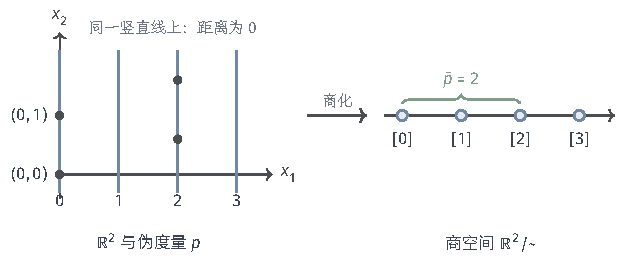
\includegraphics[width=104.916mm]{figures/02-abstract-mathematics/01-metric-and-measure/tikz/c1-pseudometric-quotient/figure.pdf}
  \caption{伪度量$p(\bm x,\bm y)=|x_1-y_1|$与商度量。左侧同一条竖直线上的点（如$(0,0)$与$(0,1)$）相互距离为零，构成一个等价类；右侧每条竖直线成为实轴上的一个点，两类之间的距离是横坐标之差，例如$|2-0|=2$。}
  \label{fig:metric-pseudometric-quotient}
\end{figure}

\section{开闭集与邻近关系}
\label{sec:metric-open-closed}

度量给出的是两点之间的数值。要谈“一点附近”“集合的边缘”“用少数点代表整个空间”，需要把这些数值组织成关于集合的判断。本节先用开球描述一点附近允许怎样移动，再由此定义开集与闭集，接着用内部、闭包与边界刻画点相对集合的位置，最后讨论能否用可数个代表点逼近空间中的每一点。本节始终固定一个度量空间$(X,d)$。

\subsection{开球与邻域}
\label{sec:metric-balls}

在实轴上，“$x$离$a$不到$r$”就是$x\in(a-r,a+r)$。一般度量空间中没有区间，但同样可以把与中心距离小于$r$的点收集起来。

\begin{definition}[开球与邻域]
\label{def:metric-open-ball}
对$a\in X$与$r>0$，集合$B(a,r)=\{x\in X:d(x,a)<r\}$称为以$a$为中心、$r$为半径的\term{开球}（open ball）。若$V\subseteq X$包含某个开球$B(a,r)$，就称$V$是$a$的一个\term{邻域}（neighborhood）。
\end{definition}

定义中的不等号是严格的，半径必须为正，因此中心本身总在球内。邻域只要求在$a$周围留出一个球的余量：实轴上的$[0,1]$是$1/2$的邻域，因为$B(1/2,1/2)=(0,1)\subseteq[0,1]$；它却不是$0$的邻域，因为每个$(-r,r)$都含有负数。

\paragraph{球的形状由度量决定}
“球”只是一个名称，它的形状完全由度量决定。在$\mathbb R^2$中，单位球$B(\bm 0,1)$在$d_2$下是圆盘内部，在$d_\infty$下是边与坐标轴平行的正方形内部$\{\bm x:|x_1|<1,|x_2|<1\}$，在$d_1$下是以四个坐标轴上的点$(\pm1,0)$、$(0,\pm1)$为顶点的菱形内部。由$\lVert\bm x\rVert_\infty\leq\lVert\bm x\rVert_2\leq\lVert\bm x\rVert_1$，三个单位球依次嵌套：$d_1$的菱形最小，$d_\infty$的正方形最大，见图~\ref{fig:metric-unit-balls}。在离散度量下，半径不超过$1$的球只含中心一个点，与“圆”毫无相似之处。

\begin{figure}[!htbp]
  \centering
  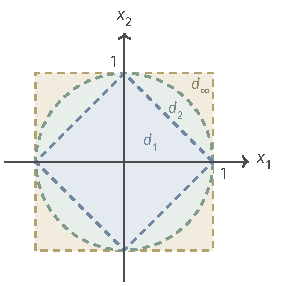
\includegraphics[width=48.055mm]{figures/02-abstract-mathematics/01-metric-and-measure/tikz/c1-unit-balls/figure.pdf}
  \caption{$\mathbb R^2$中以原点为中心的单位开球在三种度量下的形状。最内的菱形是$d_1$单位球，中间的圆盘是$d_2$单位球，最外的正方形是$d_\infty$单位球；虚线边界不属于开球。嵌套顺序对应$\lVert\bm x\rVert_\infty\leq\lVert\bm x\rVert_2\leq\lVert\bm x\rVert_1$：距离读数越大，同一半径的球越小。}
  \label{fig:metric-unit-balls}
\end{figure}

\paragraph{球内每点都有更小的球}
若$y\in B(a,r)$，令$\rho=r-d(y,a)>0$。对任意$z\in B(y,\rho)$，三角不等式给出$d(z,a)\leq d(z,y)+d(y,a)<\rho+d(y,a)=r$，所以
\begin{equation}
\label{eq:metric-ball-inside-ball}
  B(y,\rho)\subseteq B(a,r).
\end{equation}
也就是说，开球中的每一点自己也有一个留在球内的小球，这是下一小节证明“开球是开集”的依据。

\paragraph{相对开球}
设$A\subseteq X$配备子空间度量。为区分所在空间，把$A$中的开球记为$B_A(a,r)$，把$X$中的开球记为$B_X(a,r)$。对$a\in A$与$r>0$，
\begin{equation}
\label{eq:metric-relative-ball}
  B_A(a,r)=A\cap B_X(a,r),
\end{equation}
因为两边都恰好由“属于$A$且与$a$的距离小于$r$”的点组成，而子空间中的距离数值与$X$中相同。取$A=[0,1]\subseteq\mathbb R$与端点$0$，当$0<r\leq1$时，$B_A(0,r)=[0,1]\cap(-r,r)=[0,r)$。于是$[0,1/2)$在$A$中是$0$的邻域，在$\mathbb R$中却不是。图~\ref{fig:metric-relative-ball}画出了这个交集。判断邻域时，必须先说明当前所在的空间。

\begin{figure}[!htbp]
  \centering
  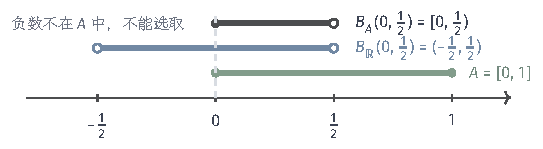
\includegraphics[width=91.934mm]{figures/02-abstract-mathematics/01-metric-and-measure/tikz/c1-relative-ball/figure.pdf}
  \caption{子空间中的相对开球。环境空间$\mathbb R$中的球$B_{\mathbb R}(0,r)=(-r,r)$（蓝色）伸到负半轴，而负数不属于子空间$A=[0,1]$（绿色）；二者的交集就是$A$中的球$B_A(0,r)=[0,r)$，它包含端点$0$。图中取$r=1/2$。}
  \label{fig:metric-relative-ball}
\end{figure}

\subsection{开集与闭集}
\label{sec:metric-open-sets}

邻域描述的是单个点。若一个集合是其中每一点的邻域，集合中的点无论在哪里，都可以向各个方向稍作移动而不离开它。

\begin{definition}[开集与闭集]
\label{def:metric-open-closed}
若对每个$x\in U$都存在$r>0$使$B(x,r)\subseteq U$，就称$U\subseteq X$为\term{开集}（open set）。若$X\setminus F$是开集，就称$F\subseteq X$为\term{闭集}（closed set）。
\end{definition}

半径可以随点改变，越靠近边缘的点可用的球越小。由式~\eqref{eq:metric-ball-inside-ball}，每个开球都是开集。空集没有需要检查的点，所以是开集；$X$包含它的每个球，所以也是开集。二者互为补集，因此它们同时也是闭集。

\begin{theorem}[开集与闭集的运算]
\label{thm:metric-open-operations}
任意多个开集的并是开集，有限多个开集的交是开集；任意多个闭集的交是闭集，有限多个闭集的并是闭集。
\end{theorem}

\begin{proof}
设$\{U_\alpha\}$是一族开集，$x\in\bigcup_\alpha U_\alpha$。则$x$属于某个$U_\beta$，存在$r>0$使$B(x,r)\subseteq U_\beta\subseteq\bigcup_\alpha U_\alpha$，所以并集是开集。

设$U_1,\dots,U_k$是开集，$x\in\bigcap_{i=1}^kU_i$。对每个$i$取$r_i>0$使$B(x,r_i)\subseteq U_i$，令$r=\min_ir_i$。由于只有有限个正数，$r>0$，而且$B(x,r)\subseteq B(x,r_i)\subseteq U_i$对每个$i$成立，所以$B(x,r)\subseteq\bigcap_iU_i$。

闭集的两条结论由补集关系得到：$X\setminus\bigcap_\alpha F_\alpha=\bigcup_\alpha(X\setminus F_\alpha)$是开集的并，$X\setminus\bigcup_{i=1}^kF_i=\bigcap_{i=1}^k(X\setminus F_i)$是有限个开集的交。
\end{proof}

证明中“有限”的作用在于取最小值时得到正数；对无限多个半径，下确界可能是零。例如每个$(-1/n,1/n)$都是$\mathbb R$中的开集，它们的交却是$\{0\}$，不是开集，因为$0$的每个球都含有非零数。同理，每个$[1/n,1]$都是闭集，它们的并$(0,1]$却不是闭集：补集$(-\infty,0]\cup(1,\infty)$在点$0$处没有留在其中的球。

\paragraph{开与闭不是互斥的两类}
“不开”不意味着“闭”。$X$与$\varnothing$既开又闭；实轴上的$[0,1)$既不开也不闭：$0\in[0,1)$没有留在其中的球，所以它不是开集；$1$在补集中，但每个$B(1,r)$都含有$[0,1)$中的点，所以补集不是开集。

\paragraph{子空间中的开集与闭集}
开与闭还取决于所在空间。由式~\eqref{eq:metric-relative-ball}可以把子空间中的开集化为环境空间的开集。

\begin{lemma}[子空间的开集与闭集]
\label{lem:metric-relative-open}
设$A\subseteq X$配备子空间度量。$U\subseteq A$是$A$中的开集，当且仅当存在$X$中的开集$V$使$U=A\cap V$；$F\subseteq A$是$A$中的闭集，当且仅当存在$X$中的闭集$C$使$F=A\cap C$。
\end{lemma}

\begin{proof}
若$U=A\cap V$且$V$在$X$中开，对$x\in U$取$r>0$使$B_X(x,r)\subseteq V$，则$B_A(x,r)=A\cap B_X(x,r)\subseteq A\cap V=U$，所以$U$在$A$中开。反过来，若$U$在$A$中开，对每个$x\in U$取$r_x>0$使$B_A(x,r_x)\subseteq U$，令$V=\bigcup_{x\in U}B_X(x,r_x)$。$V$是开球的并，在$X$中开；并且$A\cap V=\bigcup_{x\in U}B_A(x,r_x)$，它包含每个$x\in U$，又包含于$U$，所以等于$U$。

对闭集，$F$在$A$中闭当且仅当$A\setminus F$在$A$中开，即$A\setminus F=A\cap V$对某个$X$中的开集$V$成立；这又等价于$F=A\cap(X\setminus V)$，其中$X\setminus V$在$X$中闭。
\end{proof}

例如在子空间$A=[0,1]$中，$[0,1/2)=A\cap(-1,1/2)$与$(1/2,1]=A\cap(1/2,2)$都是开集，尽管它们在$\mathbb R$中都不是开集；$[0,1/2]=A\cap[-1,1/2]$是$A$中的闭集。$A$本身在$A$中既开又闭，这与它在$\mathbb R$中只闭不开并不矛盾。

\subsection{内部、闭包与边界}
\label{sec:metric-closure}

同一族开球还可以对单个点相对集合的位置分类：点可能深入集合内部，可能紧贴集合，也可能同时贴着集合与它的补集。

\begin{definition}[内部、闭包与边界]
\label{def:metric-closure}
设$A\subseteq X$。若存在$r>0$使$B(x,r)\subseteq A$，称$x$为$A$的内点，全部内点组成$A$的\term{内部}（interior），记作$A^\circ$。若对每个$r>0$都有$B(x,r)\cap A\neq\varnothing$，称$x$为$A$的闭包点，全部闭包点组成$A$的\term{闭包}（closure），记作$\overline A$。若对每个$r>0$，$B(x,r)$既与$A$相交又与$X\setminus A$相交，称$x$为$A$的边界点，全部边界点组成$A$的\term{边界}（boundary），记作$\partial A$。
\end{definition}

三个定义的区别在量词：内点要求“存在一个球”留在集合内，闭包点要求“每个球”都碰到集合，边界点要求“每个球”同时碰到两侧。按定义$A^\circ\subseteq A\subseteq\overline A$，因为$x\in A$时每个球都含有$x$本身。图~\ref{fig:metric-interior-closure-boundary}画出了三类位置。

\begin{figure}[!htbp]
  \centering
  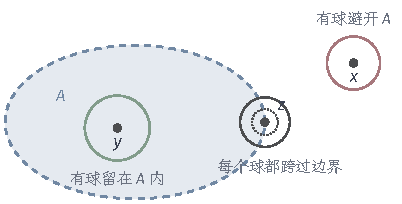
\includegraphics[width=68.104mm]{figures/02-abstract-mathematics/01-metric-and-measure/tikz/c1-interior-closure-boundary/figure.pdf}
  \caption{点相对集合$A$（浅蓝区域，虚线边界不属于$A$）的三种位置。内点$y$有一个完全落在$A$中的球；边界点$z$的每个球都同时碰到$A$与补集，它在$\overline A$中却可以不属于$A$；点$x$有一个完全避开$A$的球，所以$x\notin\overline A$。}
  \label{fig:metric-interior-closure-boundary}
\end{figure}

\paragraph{边界等于闭包去掉内部}
$x\notin A^\circ$恰好表示没有球留在$A$中，即每个球都碰到$X\setminus A$。所以边界点就是“既是闭包点、又不是内点”的点：
\begin{equation}
\label{eq:metric-boundary}
  \partial A=\overline A\setminus A^\circ.
\end{equation}
在$\mathbb R$中，$(0,1)$与$[0,1]$的内部都是$(0,1)$，闭包都是$[0,1]$，边界都是$\{0,1\}$：边界点可以属于集合，也可以不属于集合。有理数集$\mathbb Q$的情形更极端：每个区间都同时含有有理数和无理数，所以$\mathbb Q^\circ=\varnothing$、$\overline{\mathbb Q}=\mathbb R$、$\partial\mathbb Q=\mathbb R$。

\paragraph{闭包是闭集}
若$x\notin\overline A$，存在$r>0$使$B(x,r)\cap A=\varnothing$。对$y\in B(x,r)$，取$\rho=r-d(x,y)$，由式~\eqref{eq:metric-ball-inside-ball}，$B(y,\rho)\subseteq B(x,r)$也避开$A$，所以$y\notin\overline A$。于是$X\setminus\overline A$包含其每一点的一个球，是开集。由此得到：$A$是闭集当且仅当$A=\overline A$。若$A$闭而$x\notin A$，则$x$属于开集$X\setminus A$，有一个避开$A$的球，$x\notin\overline A$，故$\overline A\subseteq A$；反过来，$A=\overline A$时$A$就是闭集。对内部有对称的结论：$A^\circ$是开集，$A$开当且仅当$A=A^\circ$；论证只需把“避开$A$”换成“留在$A$内”。

\paragraph{点到集合的距离}
“每个球都碰到$A$”还可以写成一个数值条件。对非空集合$A$，定义点$x$到$A$的距离
\begin{equation}
\label{eq:metric-distance-to-set}
  d(x,A)=\inf_{a\in A}d(x,a).
\end{equation}
它是有限的非负数，因为任取$a_0\in A$都有$0\leq d(x,A)\leq d(x,a_0)$。由下确界的定义，对任意$\varepsilon>0$都有$a\in A$使$d(x,a)<d(x,A)+\varepsilon$。

\begin{lemma}[距离为零与闭包]
\label{lem:metric-distance-closure}
设$A\subseteq X$非空。则$x\in\overline A$当且仅当$d(x,A)=0$。
\end{lemma}

\begin{proof}
若$d(x,A)=0$，对每个$r>0$，由下确界的逼近性质有$a\in A$使$d(x,a)<r$，即$B(x,r)\cap A\neq\varnothing$，所以$x\in\overline A$。反过来，若$x\in\overline A$，对每个$r>0$有$a\in B(x,r)\cap A$，于是$d(x,A)\leq d(x,a)<r$；$r$任意，故$d(x,A)=0$。
\end{proof}

距离为零只说明$x$紧贴$A$，并不说明$x\in A$：$d(0,(0,1))=0$，而$0\notin(0,1)$。下确界也不一定由$A$中的某个“最近点”达到：$d(2,(0,1))=1$，但对每个$a\in(0,1)$都有$|2-a|>1$。什么条件能保证最近点存在，要等到第~\ref{sec:metric-continuous-maps}节讨论紧致集上的连续函数时回答。

\subsection{稠密集与可分空间}
\label{sec:metric-separable}

计算中只能存储有理数，却可以把任何实数逼近到任意精度。这说明一个较小的集合可以“代表”整个空间：它不必包含每一点，但必须与每一点任意接近。

\begin{definition}[稠密集与可分空间]
\label{def:metric-separable}
若$\overline D=X$，就称$D\subseteq X$在$X$中\term{稠密}（dense）。若$X$存在可数的稠密子集，就称$X$是\term{可分}（separable）的。
\end{definition}

按闭包的定义，$D$稠密等价于每个开球$B(x,r)$都与$D$相交：无论指定哪个位置$x$和哪个精度$r$，$D$中总有一点在该精度内代表$x$。可分性的要求更强，它要求同一套可数个代表点服务所有位置和所有精度。可数集合的概念见\BookChapterRef{chap:cardinality}{卷一“基数”章}。

\paragraph{实轴与离散空间}
在通常距离下，任意区间$(x-r,x+r)$都含有有理数，所以$\mathbb Q$在$\mathbb R$中稠密，而$\mathbb Q$可数，$\mathbb R$是可分的；同理，$\mathbb Q^d$在$(\mathbb R^d,d_2)$中稠密，因为对每个坐标取误差小于$r/\sqrt d$的有理数，所得点的欧氏误差小于$r$。另一方面，在不可数集合（例如$\mathbb R$本身）上取离散度量，每个单点集都是开球$B(x,1/2)=\{x\}$，稠密集必须与每个单点相交，只能是全空间，因而不可数，空间不可分。两个例子使用同一个底集$\mathbb R$，只因度量不同，可分性就不同。可分也不意味着空间本身可数：$\mathbb R$不可数，却有可数稠密子集$\mathbb Q$。

图~\ref{fig:metric-unit-balls}中的球形状和本节的相对球已经表明，邻近结构由度量和所在空间共同决定。下一节用这套邻近结构研究点列：给定精度后，点列的项最终能否都落进某个球内。

\section{点列收敛与完备性}
\label{sec:metric-convergence-completeness}

实数列$a_n\to a$的含义是误差$|a_n-a|$趋于零。把绝对值换成一般距离，就得到度量空间中的收敛。但这只回答了一类问题：已经有一个候选极限，检查点列是否逼近它。迭代求解、逐次逼近等问题往往事先不知道极限在哪里，只能观察点列内部的项是否越来越接近。本节先建立收敛和它与闭集的关系，再研究后一类问题，并说明怎样把缺失的极限补进空间。

\subsection{点列的收敛}
\label{sec:metric-convergence}

\begin{definition}[点列的收敛]
\label{def:metric-convergence}
设$(x_n)$是$X$中的点列，$x\in X$。若$d(x_n,x)\to0$，即对任意$\varepsilon>0$存在$N$使$n\geq N$时$d(x_n,x)<\varepsilon$，就称$(x_n)$\term{收敛}（converge）到$x$，记作$x_n\to x$，称$x$为它的极限。
\end{definition}

用开球的语言说，$x_n\to x$表示无论球$B(x,\varepsilon)$多小，点列从某项起都留在球中。实数列的情形见\BookChapterRef{chap:limits-continuity}{卷一“极限与连续”章}，那里的误差$|a_n-a|$在这里换成了$d(x_n,x)$。定义要求极限$x$属于当前空间$X$；如果所谓的极限在$X$之外，那么在$X$中这一列不收敛。

\paragraph{极限的基本性质}
三条基本性质都由三角不等式得到，区别在于各自控制的量。第一，极限唯一：若$x_n\to x$且$x_n\to y$，则$0\leq d(x,y)\leq d(x,x_n)+d(x_n,y)\to0$，故$d(x,y)=0$，$x=y$。第二，收敛列有界：取$\varepsilon=1$得到$N$，则对任意$n$，$d(x_n,x)\leq\max\{1,d(x_1,x),\dots,d(x_{N-1},x)\}$，所有项都落在以$x$为中心的一个有限半径球内。第三，子列保持原极限：若$n_1<n_2<\cdots$，则$n_k\geq k$，所以$k\geq N$时$d(x_{n_k},x)<\varepsilon$。

\paragraph{有限乘积中的收敛}
在有限乘积$X=X_1\times\cdots\times X_m$上取乘积度量$\rho_\infty$或$\rho_1$。由式~\eqref{eq:metric-product-bounds}，$d_i(x_{n,i},x_i)\leq\rho_\infty(x_n,x)\leq\rho_1(x_n,x)\leq\sum_{i=1}^md_i(x_{n,i},x_i)$，其中$x_{n,i}$表示$x_n$的第$i$个坐标。左边的不等式说明整体收敛推出每个坐标收敛；右边的不等式说明各坐标收敛时，有限个趋于零的数之和也趋于零，从而整体收敛。所以在有限乘积中，整体收敛与逐坐标收敛等价，且与选$\rho_1$还是$\rho_\infty$无关。$\mathbb R^d$上$d_1$与$d_\infty$下的收敛都等价于逐坐标收敛；由$d_\infty\leq d_2\leq d_1$，$d_2$下的收敛也是如此。

\paragraph{极限可能不在当前空间中}
取子空间$X=(0,1)$与点列$x_n=1/(n+1)$。在环境空间$\mathbb R$中，$x_n\to0$；但$0\notin X$，而极限唯一，所以$(x_n)$在$X$中没有极限。点列本身没有改变，改变的是允许作为极限的点。

\subsection{闭包与闭集的序列判据}
\label{sec:metric-sequential-closure}

闭包用“每个球都碰到集合”定义，这是关于所有半径的条件。点列把这些半径排成一列$1/n$，于是闭包点可以用集合内的点逐项逼近。

\begin{lemma}[闭包的序列判据]
\label{lem:metric-sequential-closure}
设$A\subseteq X$。则$x\in\overline A$当且仅当存在$A$中的点列$(a_n)$使$a_n\to x$。
\end{lemma}

\begin{proof}
设$x\in\overline A$。对每个$n$，球$B(x,1/n)$与$A$相交，从中取一点$a_n$，则$d(a_n,x)<1/n\to0$。反过来，设$a_n\in A$且$a_n\to x$。对任意$r>0$，存在$n$使$d(a_n,x)<r$，即$a_n\in B(x,r)\cap A$，所以每个球都与$A$相交，$x\in\overline A$。
\end{proof}

由第~\ref{sec:metric-closure}小节，$A$闭当且仅当$\overline A\subseteq A$。结合引理~\ref{lem:metric-sequential-closure}，得到闭集的序列判据：$A$是闭集，当且仅当$A$中的点列只要在$X$中收敛，其极限就属于$A$。例如$[0,1]$在$\mathbb R$中闭，而$(0,1]$不闭，因为$1/n\in(0,1]$收敛到$0\notin(0,1]$。

这个判据只承诺保留已经存在的极限，并不保证点列有极限。$\mathbb Q$在$\mathbb Q$自身中是闭集（全空间总是闭的），但下面会看到，$\mathbb Q$中有项彼此越来越近却没有极限的点列。要讨论极限的存在，需要一个不预先指定候选极限的判据。

\subsection{柯西列与完备性}
\label{sec:metric-cauchy}

用逐次逼近求解时，我们只能看到已经算出的项。若从某项起任意两项都足够接近，就有理由期望点列趋于某个极限；但这需要空间里确实有那个极限。

\begin{definition}[柯西列与完备空间]
\label{def:metric-complete}
若对任意$\varepsilon>0$存在$N$，使$m,n\geq N$时$d(x_m,x_n)<\varepsilon$，就称$(x_n)$为\term{柯西列}（Cauchy sequence）。若$X$中的每个柯西列都收敛到$X$中的某点，就称$(X,d)$是\term{完备}（complete）的，也称完备度量空间。
\end{definition}

柯西条件只涉及点列自身的项，不涉及任何候选极限。收敛列一定是柯西列：若$x_n\to x$，对$\varepsilon>0$取$N$使$n\geq N$时$d(x_n,x)<\varepsilon/2$，则$m,n\geq N$时$d(x_m,x_n)\leq d(x_m,x)+d(x,x_n)<\varepsilon$。反过来不一定成立，结论取决于空间。

\begin{example}[有理数中不收敛的柯西列]
\label{ex:metric-rational-cauchy}
令$q_n$为$\sqrt2$的十进制展开截到小数点后第$n$位，即$q_0=1$、$q_1=1.4$、$q_2=1.41$、$q_3=1.414$、$q_4=1.4142$，以此类推。每个$q_n$都是有理数，并且$q_n\leq\sqrt2<q_n+10^{-n}$。当$m\geq n$时，$q_m$与$q_n$的前$n$位相同，所以$0\leq q_m-q_n<10^{-n}$，$(q_n)$是$\mathbb Q$中（通常距离下）的柯西列。在$\mathbb R$中$q_n\to\sqrt2$，而$\sqrt2$是无理数；由极限唯一性，$(q_n)$在$\mathbb Q$中没有极限。所以$\mathbb Q$不完备。图~\ref{fig:metric-rational-cauchy}画出了这些项向$\sqrt2$处的“空缺”聚拢的情形。
\end{example}

\begin{figure}[!htbp]
  \centering
  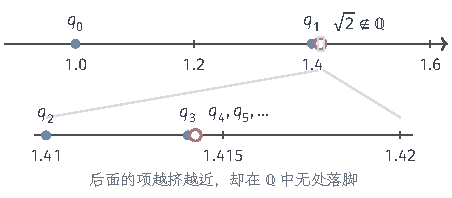
\includegraphics[width=76.616mm]{figures/02-abstract-mathematics/01-metric-and-measure/tikz/c1-rational-cauchy/figure.pdf}
  \caption{有理数中不收敛的柯西列。上方数轴上的蓝点是$\sqrt2$的十进制截断$1,\ 1.4,\ 1.41,\ 1.414$，空心圆标出$\sqrt2\approx1.41421$，它不属于$\mathbb Q$；下方放大$[1.41,1.42]$一段，可见后面的项继续向空心圆聚拢。从第$n$项起任意两项相差不到$10^{-n}$，但在$\mathbb Q$中找不到它们的极限。}
  \label{fig:metric-rational-cauchy}
\end{figure}

\paragraph{实数与欧氏空间的完备性}
实数在通常距离下是完备的，这正是卷一“极限与连续”章中的柯西收敛准则，它依赖实数的确界性质。由此可以得到$\mathbb R^d$的完备性：若$(\bm x_n)$在$d_2$下是柯西列，由$|x_{m,i}-x_{n,i}|\leq d_2(\bm x_m,\bm x_n)$，每个坐标都是实数柯西列，各自收敛到某个$x_i$；令$\bm x=(x_1,\dots,x_d)$，由上一小节，逐坐标收敛推出$d_2(\bm x_n,\bm x)\to0$。同样的论证适用于$d_1$与$d_\infty$。

\paragraph{完备子集与闭子集}
完备性与闭性之间有两个方向不同的结论，前者需要环境空间完备，后者对任意度量空间成立。

\begin{theorem}[完备性与闭集]
\label{thm:metric-complete-closed}
设$A\subseteq X$配备子空间度量。
\begin{enumerate}
  \item 若$X$完备且$A$在$X$中闭，则$A$完备。
  \item 若$A$完备，则$A$在$X$中闭。
\end{enumerate}
\end{theorem}

\begin{proof}
(1) 设$(a_n)$是$A$中的柯西列。子空间距离与$X$中的距离相同，所以它也是$X$中的柯西列，由$X$完备，存在$x\in X$使$a_n\to x$。$A$闭，由闭集的序列判据，$x\in A$，所以$(a_n)$在$A$中收敛。

(2) 设$a_n\in A$且在$X$中$a_n\to x$。收敛列是柯西列，所以$(a_n)$是$A$中的柯西列；$A$完备，存在$a\in A$使$a_n\to a$。在$X$中极限唯一，故$x=a\in A$。由闭集的序列判据，$A$闭。
\end{proof}

于是$[0,1]$在通常距离下完备，而$(0,1)$不完备：后者在$\mathbb R$中不闭，由结论(2)不可能完备。结论(1)中的完备性假设不能省去：$\mathbb Q$在$\mathbb Q$中闭，却不完备。

\paragraph{有限乘积的完备性}
设$(X_i,d_i)$都完备，$X=X_1\times\cdots\times X_m$取$\rho_\infty$。若$(x_n)$是$X$中的柯西列，由$d_i(x_{m,i},x_{n,i})\leq\rho_\infty(x_m,x_n)$，每个坐标列都是$X_i$中的柯西列，收敛到某个$x_i\in X_i$；再由逐坐标收敛等价于整体收敛，$x_n\to(x_1,\dots,x_m)$。所以有限个完备空间的乘积仍完备，对$\rho_1$亦然。上一段$\mathbb R^d$的完备性是它的特例。

\subsection{度量空间的完备化}
\label{sec:metric-completion}

$\mathbb Q$的柯西列“想要”收敛到的点，正是实数。能否对一般度量空间做同样的事：用柯西列代表缺失的极限，构造一个完备空间，使原空间稠密地放在其中，且原有距离不变？答案是肯定的，构造恰好用到第~\ref{sec:metric-pseudometric}小节的商度量。

\paragraph{用柯西列代表新点}
设$\mathcal C$是$X$中全部柯西列组成的集合。对$(x_n),(y_n)\in\mathcal C$，由反向三角不等式~\eqref{eq:metric-reverse-triangle}使用两次，
\[
  \begin{aligned}
    \bigl|d(x_m,y_m)-d(x_n,y_n)\bigr|
    &\leq\bigl|d(x_m,y_m)-d(x_n,y_m)\bigr|\\
    &\quad+\bigl|d(x_n,y_m)-d(x_n,y_n)\bigr|\\
    &\leq d(x_m,x_n)+d(y_m,y_n).
  \end{aligned}
\]
右边在$m,n\to\infty$时趋于零，所以$\bigl(d(x_n,y_n)\bigr)$是实数柯西列。由实数的完备性，极限
\[
  D\bigl((x_n),(y_n)\bigr)=\lim_{n\to\infty}d(x_n,y_n)
\]
存在。$D$非负、对称，并且对三列逐项写出$d(x_n,z_n)\leq d(x_n,y_n)+d(y_n,z_n)$后取极限，得到三角不等式。但两列不同的柯西列可能有$D=0$，例如$(1/n)$与$(-1/n)$，所以$D$只是$\mathcal C$上的伪度量。按第~\ref{sec:metric-pseudometric}小节，把$D=0$的柯西列识别为同一点，得到商集$\widehat X=\mathcal C/{\sim}$及其上的度量$\hat d$。两列的距离趋于零，意味着它们“想要趋于同一点”，识别它们正符合这一直观。

\paragraph{原空间的等距嵌入}
对$x\in X$，常值列$(x,x,\dots)$是柯西列，令$\iota(x)$为它的等价类。则$\hat d(\iota(x),\iota(y))=\lim_nd(x,y)=d(x,y)$，所以$\iota$保持距离，原空间连同它的度量被原样放进$\widehat X$。$\iota(X)$在$\widehat X$中稠密：设$\xi\in\widehat X$由柯西列$(x_n)$代表，对$\varepsilon>0$取$N$使$m,n\geq N$时$d(x_m,x_n)<\varepsilon$，则对$m\geq N$，$\hat d(\iota(x_m),\xi)=\lim_nd(x_m,x_n)\leq\varepsilon$。

\begin{theorem}[完备化]
\label{thm:metric-completion}
$(\widehat X,\hat d)$是完备度量空间，$\iota:X\to\widehat X$保持距离，且$\iota(X)$在$\widehat X$中稠密。称$\widehat X$为$X$的\term{完备化}（completion）。
\end{theorem}

\begin{proof}
度量性与嵌入的两条性质已在上面证明，只剩完备性。设$(\xi_k)$是$\widehat X$中的柯西列。由稠密性，对每个$k$取$x_k\in X$使$\hat d(\iota(x_k),\xi_k)<1/k$。因为$\iota$保持距离，
\[
  d(x_k,x_l)=\hat d(\iota(x_k),\iota(x_l))<\frac1k+\hat d(\xi_k,\xi_l)+\frac1l,
\]
右边在$k,l\to\infty$时趋于零，所以$(x_k)$是$X$中的柯西列，它代表$\widehat X$中的一点$\xi$。最后，
\[
  \hat d(\xi_k,\xi)\leq\hat d(\xi_k,\iota(x_k))+\hat d(\iota(x_k),\xi)<\frac1k+\lim_{l\to\infty}d(x_k,x_l).
\]
对$\varepsilon>0$，当$k$充分大时，$1/k<\varepsilon$，且对一切充分大的$l$有$d(x_k,x_l)<\varepsilon$，所以右边小于$2\varepsilon$。因此$\xi_k\to\xi$。
\end{proof}

这一构造的要点是：保留原来的距离，并稠密地补入全部缺失的极限。对$X=\mathbb Q$，把有理柯西列$(q_n)$所代表的点对应到它在$\mathbb R$中的极限：$D=0$的两列有相同的实数极限，所以这个对应良定义；$|\lim q_n-\lim r_n|=\lim|q_n-r_n|$说明它保持距离；每个实数都是其十进制截断的极限，所以它是满射。于是$\widehat{\mathbb Q}$与$\mathbb R$之间有保持距离的双射。对已经完备的$X$，每个柯西列都已有极限，$\iota$是满射，完备化不增加新点。完备化在保持距离的意义下唯一，证明需要把等距映射从稠密子集延拓到整个空间，这里不展开。

\section{紧致性}
\label{sec:metric-compactness}

实轴上的闭区间有两条重要性质：其中的数列总有收敛子列，连续函数在其上取得最大值和最小值。开区间$(0,1)$和整条实轴都没有这些性质。本节寻找一般度量空间中与“闭区间”对应的条件。它的核心是有限性：无论精度多高，集合都能由有限个小球控制。我们先从覆盖的角度提出这一要求，再把它与收敛子列、完备性联系起来。

\subsection{有界集与全有界集}
\label{sec:metric-totally-bounded}

“集合不太大”最直接的说法是：它能装进一个有限半径的球中。

\begin{definition}[有界集]
\label{def:metric-bounded}
若存在$a\in X$与$R<\infty$使$A\subseteq B(a,R)$，就称$A\subseteq X$是\term{有界}（bounded）的。非空集合$A$的\term{直径}（diameter）定义为$\operatorname{diam}A=\sup_{x,y\in A}d(x,y)$。
\end{definition}

两种说法等价：若$A\subseteq B(a,R)$，三角不等式给出$d(x,y)\leq d(x,a)+d(a,y)<2R$，所以$\operatorname{diam}A\leq2R$；反过来，若$\operatorname{diam}A<\infty$，任取$a\in A$，则$A\subseteq B(a,\operatorname{diam}A+1)$。

有界只控制集合的总体范围，不控制集合的内部能否在细尺度下被少量信息描述。离散度量下的无限集合$X$直径为$1$，因而有界；但用半径$1/2$的球覆盖它时，每个球只含一个点，需要无限多个球。下面的定义要求每个尺度都只需有限个球。

\begin{definition}[全有界与$\varepsilon$网]
\label{def:metric-totally-bounded}
设$A\subseteq X$，$\varepsilon>0$。若有限集$\{a_1,\dots,a_k\}\subseteq A$满足$A\subseteq\bigcup_{i=1}^kB(a_i,\varepsilon)$，就称它是$A$的一个有限$\varepsilon$网（finite $\varepsilon$-net），不指明精度时简称\term{有限网}。若对每个$\varepsilon>0$，$A$都有有限$\varepsilon$网，就称$A$是\term{全有界}（totally bounded）的。
\end{definition}

$\varepsilon$网中的点是在精度$\varepsilon$下代表$A$的有限个样本：$A$中每一点都与某个代表点相距不到$\varepsilon$。代表点的个数和位置可以随$\varepsilon$改变，精度越高通常需要越多代表点，但对每个精度都必须是有限个。图~\ref{fig:metric-epsilon-net}画出了同一个集合在两种精度下的网。

\begin{figure}[!htbp]
  \centering
  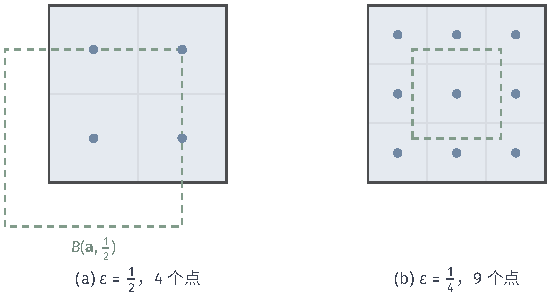
\includegraphics[width=93.169mm]{figures/02-abstract-mathematics/01-metric-and-measure/tikz/c1-epsilon-net/figure.pdf}
  \caption{正方形$[0,1]^2$在$d_\infty$下的有限$\varepsilon$网。把正方形等分为小格，蓝点取在各小格中心，小格中的点与该格中心的$d_\infty$距离至多为半个格宽。(a) $\varepsilon=1/2$时用$4$个点$\bigl((2i-1)/4,(2j-1)/4\bigr)$，格内距离至多$1/4<1/2$；虚线正方形是其中一个球$B(\bm a,1/2)$。(b) $\varepsilon=1/4$时用$9$个点$\bigl((2i-1)/6,(2j-1)/6\bigr)$，格内距离至多$1/6<1/4$。精度提高时代表点增多，但始终是有限个。}
  \label{fig:metric-epsilon-net}
\end{figure}

\paragraph{全有界推出有界与可分}
全有界比有界强。取一个有限$1$网$\{a_1,\dots,a_k\}$，任意$x,y\in A$分别落在某个$B(a_i,1)$与$B(a_j,1)$中，于是$d(x,y)<2+\max_{i,j}d(a_i,a_j)$，$A$有界。全有界还推出$A$（作为子空间）可分：对每个$n$取一个有限$1/n$网$F_n$，令$D=\bigcup_nF_n$，它是可数个有限集的并，因而可数。对任意$x\in A$与$r>0$，取$n>1/r$，$F_n$中有一点与$x$相距小于$1/n<r$，所以$D$在$A$中稠密。

\paragraph{三个要求的区别}
两个反例说明这些蕴含不能反过来。无限离散空间有界，但对$\varepsilon=1/2$没有有限网，因而不全有界。通常距离下的$\mathbb R$可分（有可数稠密集$\mathbb Q$），却无界，也就不全有界。有界控制总体范围，可分要求一套可数代表服务于所有精度，全有界则要求每个精度下只需有限个代表；三者各自约束不同的东西。

\subsection{开覆盖与紧致集}
\label{sec:metric-open-cover}

全有界允许我们为每个精度挑选最方便的一组球。有些论证中，球不是我们挑的，而是别人给定的一族开集，例如“每一点各自有一个让函数变化不大的邻域”。紧致性要求：无论给定怎样的开覆盖，都能从中选出有限个成员完成覆盖。

\begin{definition}[紧致集]
\label{def:metric-compact}
若一族开集$\{U_\alpha\}_{\alpha\in I}$满足$X=\bigcup_{\alpha\in I}U_\alpha$，就称它是$X$的一个\term{开覆盖}（open cover）。若$X$的每个开覆盖都有有限子族$U_{\alpha_1},\dots,U_{\alpha_k}$仍覆盖$X$，就称度量空间$X$是\term{紧致}（compact）的。若子集$K\subseteq X$配备子空间度量后是紧致的，就称$K$是紧致集（或紧集）。
\end{definition}

由引理~\ref{lem:metric-relative-open}，$K$中的开集都形如$K\cap V$，$V$在$X$中开。所以$K$紧致，等价于：每一族满足$K\subseteq\bigcup_\alpha V_\alpha$的$X$中的开集都有有限子族仍覆盖$K$。定义中的“有限子覆盖”必须从给定的覆盖中挑选，不能另换一组更方便的开集；正是这一点使紧致性比全有界强。

\paragraph{紧致集全有界且闭}
把全部半径为$\varepsilon$的球$\{B_K(x,\varepsilon):x\in K\}$作为开覆盖代入定义，有限子覆盖的中心就是一个有限$\varepsilon$网，所以紧致集全有界。紧致集还在任何环境空间中都是闭集。设$x\in X\setminus K$。对每个$y\in K$，令$r_y=d(x,y)/2>0$，开球$B(y,r_y)$覆盖$K$，取有限子覆盖$B(y_1,r_{y_1}),\dots,B(y_k,r_{y_k})$，令$r=\min_ir_{y_i}>0$。若$z\in B(x,r)\cap B(y_i,r_{y_i})$，则$d(x,y_i)\leq d(x,z)+d(z,y_i)<r+r_{y_i}\leq2r_{y_i}=d(x,y_i)$，矛盾；所以$B(x,r)$与$K$不交。外点都有避开$K$的球，$K$闭。

\begin{example}[全有界而不紧致]
\label{ex:metric-open-interval-cover}
$(0,1)$在通常距离下全有界：对$\varepsilon>0$，取有限个间距小于$\varepsilon$的点即可。但$(0,1)$不紧致。令$U_n=(1/n,1)$（$n\geq2$），每一点$x\in(0,1)$在$n>1/x$时属于$U_n$，所以$\{U_n\}$覆盖$(0,1)$。任取有限个$U_{n_1},\dots,U_{n_k}$，它们的并是$(1/N,1)$，其中$N=\max_in_i$，它漏掉了$(0,1/N]$中的点。图~\ref{fig:metric-open-cover-interval}画出了这个覆盖。用有限个小球覆盖$(0,1)$并不困难，难点在于这个给定覆盖的成员越来越靠近$0$而永远不包含它附近的全部点。
\end{example}

\begin{figure}[!htbp]
  \centering
  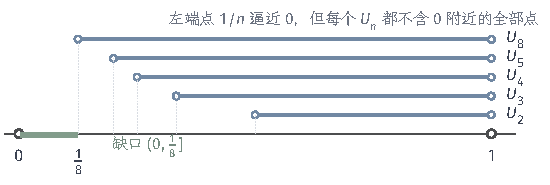
\includegraphics[width=93.105mm]{figures/02-abstract-mathematics/01-metric-and-measure/tikz/c1-open-cover/figure.pdf}
  \caption{开区间$(0,1)$的一个没有有限子覆盖的开覆盖。各条蓝色线段是$U_n=(1/n,1)$，$n=2,3,4,5,8$，它们的左端点$1/n$逐渐逼近$0$却不到达$0$；任取有限个成员，并集是某个$(1/N,1)$，在$0$附近留下绿色标出的缺口$(0,1/N]$。}
  \label{fig:metric-open-cover-interval}
\end{figure}

无限离散空间提供了另一类反例：它闭（作为全空间）且有界，但全部单点开球$\{\{x\}\}$组成开覆盖，任何有限子族只覆盖有限个点，所以不紧致。在一般度量空间中，“闭且有界”不足以推出紧致。

\subsection{紧致性的序列刻画}
\label{sec:metric-sequential-compactness}

闭区间上“数列有收敛子列”的性质也可以作为紧致性的定义。在度量空间中，它与开覆盖的定义等价。

\begin{definition}[序列紧致]
\label{def:metric-sequentially-compact}
若$K$中的每个点列都有在$K$中收敛的子列，就称$K\subseteq X$是\term{序列紧致}（sequentially compact）的。
\end{definition}

\begin{theorem}[紧致性的序列刻画]
\label{thm:metric-compact-sequential}
度量空间的子集$K$紧致，当且仅当它序列紧致。
\end{theorem}

\begin{proof}
\emph{紧致推出序列紧致。}设$K$紧致，$(x_n)$是$K$中的点列。先证明存在$y\in K$，使每个球$B(y,r)$都含有点列中下标无限多的项。若不然，每个$y\in K$都有半径$r_y>0$，使$B(y,r_y)$只含有限个下标$n$的$x_n$。这些球覆盖$K$，取有限子覆盖$B(y_1,r_{y_1}),\dots,B(y_k,r_{y_k})$。每个$x_n$都在其中某个球内，而每个球只容纳有限个下标，于是下标总数有限，与点列有无限多个下标矛盾。

再由这样的$y$构造收敛子列。取$n_1$使$x_{n_1}\in B(y,1)$；设已取$n_1<\cdots<n_k$，由于$B(y,1/(k+1))$含有下标无限多的项，可以取$n_{k+1}>n_k$使$x_{n_{k+1}}\in B(y,1/(k+1))$。于是$d(x_{n_k},y)<1/k\to0$，子列在$K$中收敛到$y$。

\emph{序列紧致推出紧致。}设$K$序列紧致。第一步证明$K$全有界。若对某个$\varepsilon>0$没有有限$\varepsilon$网，任取$x_1\in K$；设已取$x_1,\dots,x_n$，它们不是$\varepsilon$网，所以有$x_{n+1}\in K$不在$\bigcup_{i\leq n}B(x_i,\varepsilon)$中。所得点列两两距离至少为$\varepsilon$，它的任何子列都不是柯西列，也就不收敛，与序列紧致矛盾。

第二步证明：对$K$的任意开覆盖$\{U_\alpha\}$，存在$\delta>0$，使每个$x\in K$的球$B_K(x,\delta)$都包含于某个$U_\alpha$。若不然，对每个$n$都有$x_n\in K$，使$B_K(x_n,1/n)$不包含于任何$U_\alpha$。取子列$x_{n_k}\to x\in K$。$x$属于某个$U_\beta$，又因$U_\beta$在$K$中开，有$r>0$使$B_K(x,r)\subseteq U_\beta$。取$k$充分大，使$d(x_{n_k},x)<r/2$且$1/n_k<r/2$。对$z\in B_K(x_{n_k},1/n_k)$有$d(z,x)<1/n_k+r/2<r$，所以$B_K(x_{n_k},1/n_k)\subseteq B_K(x,r)\subseteq U_\beta$，矛盾。

第三步完成覆盖。由第一步取有限$\delta$网$\{a_1,\dots,a_m\}$，由第二步每个$B_K(a_i,\delta)$包含于某个$U_{\alpha_i}$。这些球覆盖$K$，所以$U_{\alpha_1},\dots,U_{\alpha_m}$覆盖$K$。
\end{proof}

第二步得到的$\delta$称为该覆盖的\term{Lebesgue数}（Lebesgue number）：只要观察范围小于$\delta$，就不必担心跨越覆盖成员的边界。整个证明反复使用距离：用$1/k$半径的球选子列，用两两距离判断子列不是柯西列，用三角不等式比较两个球。对没有度量的一般拓扑空间，紧致与序列紧致可以不等价，本章不讨论那种情形。

\subsection{完备与全有界判据}
\label{sec:metric-complete-totally-bounded}

开覆盖条件难以直接验证。下面的判据把紧致性拆成两个分别容易检查的条件：完备性保证柯西列有极限，全有界性保证能抽出柯西子列。

\begin{theorem}[紧致的完备全有界判据]
\label{thm:metric-compact-complete-tb}
度量空间$K$紧致，当且仅当$K$完备且全有界。
\end{theorem}

\begin{proof}
设$K$紧致。全有界已在第~\ref{sec:metric-open-cover}小节证明。对完备性，设$(x_n)$是$K$中的柯西列。由定理~\ref{thm:metric-compact-sequential}，有子列$x_{n_k}\to x\in K$。对$\varepsilon>0$取$N$使$m,n\geq N$时$d(x_m,x_n)<\varepsilon/2$，再取$k$使$n_k\geq N$且$d(x_{n_k},x)<\varepsilon/2$，则$n\geq N$时$d(x_n,x)\leq d(x_n,x_{n_k})+d(x_{n_k},x)<\varepsilon$。所以整个柯西列收敛到$x$。

反过来，设$K$完备且全有界，$(x_n)$是$K$中的点列。用有限个半径$1$的球覆盖$K$，其中至少有一个球含有下标无限多的项，记这些下标的集合为$I_1$。再用有限个半径$1/2$的球覆盖$K$，其中某个球含有$\{x_n:n\in I_1\}$中下标无限多的项，记这些下标为$I_2\subseteq I_1$。如此继续，得到无限下标集$I_1\supseteq I_2\supseteq\cdots$，其中$I_j$对应的项都落在同一个半径$1/j$的球中。取$n_1\in I_1$，再依次取$n_j\in I_j$且$n_j>n_{j-1}$。当$k,l\geq j$时，$x_{n_k}$与$x_{n_l}$都属于$I_j$所对应的球，故$d(x_{n_k},x_{n_l})<2/j$。子列$(x_{n_j})$是柯西列，由完备性在$K$中收敛。于是$K$序列紧致，由定理~\ref{thm:metric-compact-sequential}，$K$紧致。
\end{proof}

用这一判据重看前面的例子：$(0,1)$全有界但不完备，无限离散空间完备（其中的柯西列从某项起为常数）但不全有界，二者都不紧致；$[0,1]$完备且全有界，因而紧致。

\paragraph{欧氏空间中的闭有界集}
在$\mathbb R^d$中，有界与全有界一致，于是判据简化为熟悉的形式。

\begin{theorem}[欧氏空间的闭有界判据]
\label{thm:metric-heine-borel}
在$(\mathbb R^d,d_2)$中，子集$K$紧致当且仅当它闭且有界。
\end{theorem}

\begin{proof}
紧致集闭且有界已在第~\ref{sec:metric-open-cover}小节证明。反过来，设$K$闭且有界，则存在$M$使$K\subseteq[-M,M]^d$。$\mathbb R^d$完备而$K$闭，由定理~\ref{thm:metric-complete-closed}，$K$完备。对全有界，给定$\varepsilon>0$，取正整数$s$使边长$h=2M/s<\varepsilon/\sqrt d$，把$[-M,M]^d$等分为$s^d$个边长为$h$的闭小立方体。每个小立方体中两点的欧氏距离至多为$h\sqrt d<\varepsilon$。在每个与$K$相交的小立方体中取一点$a_Q\in K$，得到至多$s^d$个点；$K$中任一点所在的小立方体也含有对应的$a_Q$，二者距离小于$\varepsilon$。所以这些点组成$K$的有限$\varepsilon$网。由定理~\ref{thm:metric-compact-complete-tb}，$K$紧致。
\end{proof}

证明中有限维出现在网格的计数$s^d$上：维数固定时，网格点数有限。特别地，$\mathbb R$中的闭区间$[a,b]$紧致，闭区间上数列有收敛子列的性质成为定理~\ref{thm:metric-compact-sequential}的特例。在一般度量空间（包括后面要讨论的函数空间）中，闭有界集不一定紧致，必须回到“完备且全有界”来判断。

\section{连续映射}
\label{sec:metric-continuous-maps}

前面几节研究一个空间内部的点和集合。现在固定两个度量空间$(X,d_X)$、$(Y,d_Y)$和一个映射$f:D\to Y$，其中$D\subseteq X$配备子空间度量，问输入的小误差能否保证输出的小误差。本节先定义函数极限与连续性，再按“容差是否随位置变化”“输出误差能否被输入误差的固定倍数控制”区分一致连续与Lipschitz条件，最后研究紧致定义域给连续映射带来的结论。

\subsection{极限与连续性}
\label{sec:metric-limits-continuity}

讨论$x\to a$时$f(x)$的行为，要求$a$附近确实有$D$中的点可以取。若$a\in X$的每个球$B(a,r)$都含有$D$中异于$a$的点，就称$a$是$D$的\term{聚点}（accumulation point）。聚点本身不必属于$D$，例如$0$是$(0,1)$的聚点。

\begin{definition}[函数极限]
\label{def:metric-function-limit}
设$a$是$D$的聚点，$L\in Y$。若对任意$\varepsilon>0$存在$\delta>0$，使$x\in D$且$0<d_X(x,a)<\delta$时$d_Y(f(x),L)<\varepsilon$，就称$x\to a$时$f(x)$的极限为$L$，记作$\lim_{x\to a}f(x)=L$。
\end{definition}

条件$0<d_X(x,a)$排除了基点本身，所以极限只看$a$周围的取值，与$f(a)$是否有定义、取什么值无关。聚点条件保证了极限唯一：若$L$与$L'$都是极限，对$\varepsilon>0$取两个$\delta$中较小者，由聚点条件存在满足$0<d_X(x,a)<\delta$的$x\in D$，于是$d_Y(L,L')\leq d_Y(L,f(x))+d_Y(f(x),L')<2\varepsilon$；$\varepsilon$任意，故$L=L'$。若$a$不是聚点，满足$0<d_X(x,a)<\delta$的$x$可能根本不存在，定义中的条件对任何$L$都空洞地成立，这时不谈极限。

\begin{definition}[连续映射]
\label{def:metric-continuous}
设$a\in D$。若对任意$\varepsilon>0$存在$\delta>0$，使$x\in D$且$d_X(x,a)<\delta$时$d_Y(f(x),f(a))<\varepsilon$，就称$f$在$a$处\term{连续}（continuous）。若$f$在$D$的每一点都连续，就称$f$是连续映射。
\end{definition}

连续性只在定义域中的点讨论，输出目标就是$f(a)$。当$a\in D$又是$D$的聚点时，连续等价于$\lim_{x\to a}f(x)=f(a)$。若$a\in D$是孤立点，即某个球$B(a,r)$中除$a$外没有$D$中的点，取$\delta=r$，满足$d_X(x,a)<\delta$的$x$只有$a$本身，条件自动成立，所以$f$在孤立点处连续；这里用的是$x=a$本身，而不是空洞地宣称有一个穿孔极限。

\paragraph{序列判据}
连续性也可以用点列检查，这在证明中常常更方便。

\begin{theorem}[连续性的序列判据]
\label{thm:metric-sequential-continuity}
$f$在$a\in D$处连续，当且仅当对$D$中每个满足$x_n\to a$的点列，都有$f(x_n)\to f(a)$。
\end{theorem}

\begin{proof}
设$f$在$a$处连续，$x_n\to a$。对$\varepsilon>0$取连续性中的$\delta$，再取$N$使$n\geq N$时$d_X(x_n,a)<\delta$，则$n\geq N$时$d_Y(f(x_n),f(a))<\varepsilon$。反过来，若$f$在$a$处不连续，则存在$\varepsilon>0$，使对每个$\delta=1/n$都有$x_n\in D$满足$d_X(x_n,a)<1/n$而$d_Y(f(x_n),f(a))\geq\varepsilon$。于是$x_n\to a$，但$f(x_n)$不收敛到$f(a)$。
\end{proof}

\paragraph{开集原像判据与复合}
对整个映射，连续性还可以写成关于集合的条件，不必逐点选取$\delta$。

\begin{theorem}[开集原像判据]
\label{thm:metric-open-preimage}
$f:D\to Y$连续，当且仅当对$Y$中每个开集$V$，原像$f^{-1}(V)=\{x\in D:f(x)\in V\}$是$D$中的开集。若$f:D\to Y$与$g:Y\to Z$都连续，则$g\circ f$连续。
\end{theorem}

\begin{proof}
设$f$连续，$V$在$Y$中开，$a\in f^{-1}(V)$。取$\varepsilon>0$使$B_Y(f(a),\varepsilon)\subseteq V$，再取连续性中的$\delta$，则$B_D(a,\delta)$中的点都映入$B_Y(f(a),\varepsilon)\subseteq V$，即$B_D(a,\delta)\subseteq f^{-1}(V)$。所以原像是$D$中的开集。反过来，对$a\in D$与$\varepsilon>0$，开球$B_Y(f(a),\varepsilon)$的原像是含$a$的开集，其中有某个$B_D(a,\delta)$，这正是$a$处连续的定义。复合的结论由原像判据直接得到：$(g\circ f)^{-1}(W)=f^{-1}(g^{-1}(W))$，对开集$W$，$g^{-1}(W)$开，再取$f$的原像仍开。
\end{proof}

三种刻画各有用途：$\varepsilon$-$\delta$定义适合具体的误差估计，序列判据适合与收敛子列结合，原像判据只涉及集合运算。第二章定义可测映射时，会把“开集的原像是开集”改为“可测集的原像是可测集”，这里的原像判据就是它的具体参照。

\subsection{一致连续}
\label{sec:metric-uniform-continuity}

连续性的定义中，$\delta$可以依赖基点$a$。对$f(x)=x^2$在$a$处取$\varepsilon=1$，最大的可用半径是$\delta(a)=\sqrt{a^2+1}-|a|$，它满足$(|a|+\delta)^2=a^2+1$。$a=1$时$\delta=\sqrt2-1\approx0.414$，$a=3$时$\delta=\sqrt{10}-3\approx0.162$，$|a|$越大，$\delta$越小，并且$\delta(a)=1/(\sqrt{a^2+1}+|a|)\to0$。图~\ref{fig:metric-uniform-continuity}(a)画出了这一现象。若要求一个$\delta$同时适用于所有点，就得到更强的条件。

\begin{definition}[一致连续]
\label{def:metric-uniform-continuity}
若对任意$\varepsilon>0$存在$\delta>0$，使所有满足$d_X(x,y)<\delta$的$x,y\in D$都有$d_Y(f(x),f(y))<\varepsilon$，就称$f$在$D$上\term{一致连续}（uniformly continuous）。
\end{definition}

与逐点连续相比，两个定义的差别只在量词次序：逐点连续是“对每个$a$和$\varepsilon$，存在$\delta$”，$\delta$可以随$a$变化；一致连续是“对每个$\varepsilon$，存在一个$\delta$适用于全部点对”。

\begin{example}[$x^2$在不同定义域上]
\label{ex:metric-square-uniform}
在$\mathbb R$上，$x^2$不一致连续：取$x_n=n$、$y_n=n+1/n$，则$|x_n-y_n|=1/n\to0$，而$|y_n^2-x_n^2|=2+1/n^2>2$，所以对$\varepsilon=2$找不到统一的$\delta$。在$[-M,M]$上，$|x^2-y^2|=|x+y|\,|x-y|\leq2M|x-y|$，取$\delta=\varepsilon/(2M)$即可，所以$x^2$一致连续。同一个公式，定义域不同，结论不同。
\end{example}

\begin{figure*}[!htbp]
  \centering
  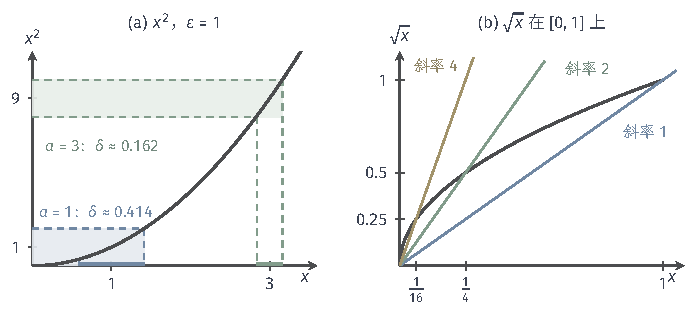
\includegraphics[width=116.695mm]{figures/02-abstract-mathematics/01-metric-and-measure/tikz/c1-uniform-continuity/figure.pdf}
  \caption{连续性中容差随位置的变化。(a) $f(x)=x^2$，取输出容差$\varepsilon=1$：在$a=1$处输入可以偏离$\sqrt2-1\approx0.414$，在$a=3$处只能偏离$\sqrt{10}-3\approx0.162$，曲线越陡，可用的输入区间越窄，在全实轴上没有统一的$\delta$。(b) $f(x)=\sqrt x$在$[0,1]$上：过点$(t,\sqrt t)$与原点的割线斜率$1/\sqrt t$在$t\to0$时无界，图中画出$t=1,\ 1/4,\ 1/16$三条割线，斜率依次为$1,\ 2,\ 4$；不存在统一的Lipschitz常数，但$\sqrt x$在$[0,1]$上仍一致连续。}
  \label{fig:metric-uniform-continuity}
\end{figure*}

\paragraph{一致连续映射保持柯西列}
若$f$一致连续而$(x_n)$是$D$中的柯西列，对$\varepsilon>0$取一致连续的$\delta$，再取$N$使$m,n\geq N$时$d_X(x_m,x_n)<\delta$，则$d_Y(f(x_m),f(x_n))<\varepsilon$，所以$(f(x_n))$是柯西列。逐点连续做不到这一点：$f(x)=1/x$在$(0,1)$上连续，柯西列$1/(n+1)$的像$n+1$却不是柯西列。另一方面，保持柯西列不等于输出有极限：恒等映射$(0,1)\to(0,1)$一致连续，柯西列$1/(n+1)$的像仍是它自己，在陪域$(0,1)$中没有极限。输出极限是否存在取决于陪域是否完备。

\subsection{Lipschitz映射}
\label{sec:metric-lipschitz}

一致连续只保证存在统一的$\delta$，没有说明$\delta$与$\varepsilon$的数量关系。很多误差估计需要更具体的结论：输出误差不超过输入误差的固定倍数。

\begin{definition}[Lipschitz映射]
\label{def:metric-lipschitz}
若存在常数$L\geq0$，使所有$x,y\in D$都满足
\[
  d_Y(f(x),f(y))\leq L\,d_X(x,y),
\]
就称$f$是\term{Lipschitz映射}（Lipschitz map），$L$称为Lipschitz常数。若每个$a\in D$都有半径$r_a>0$与常数$L_a$，使上式在$D\cap B(a,r_a)$上以$L_a$成立，就称$f$\term{局部Lipschitz}（locally Lipschitz）。
\end{definition}

全局Lipschitz推出一致连续：$L>0$时取$\delta=\varepsilon/L$，$L=0$时$f$为常值，任取$\delta$即可。局部Lipschitz推出连续：在$a$处取$\delta=\min\{r_a,\varepsilon/(L_a+1)\}$，则$d_X(x,a)<\delta$时$d_Y(f(x),f(a))\leq L_a\delta<\varepsilon$。局部常数$L_a$可以随$a$无限增大，这时没有全局常数。由反向三角不等式~\eqref{eq:metric-reverse-triangle}，对固定的$z$，$x\mapsto d_X(x,z)$是Lipschitz常数为$1$的映射；同样，由式~\eqref{eq:metric-distance-to-set}定义的$x\mapsto d_X(x,A)$也是$1$-Lipschitz的：对任意$a\in A$，$d_X(x,A)\leq d_X(x,a)\leq d_X(x,y)+d_X(y,a)$，对$a$取下确界得$d_X(x,A)\leq d_X(x,y)+d_X(y,A)$，交换$x,y$即得。

\paragraph{三种条件的区分}
两个例子说明三种条件确实不同。$\sqrt x$在$[0,1]$上一致连续：对$0\leq y\leq x$，$(\sqrt x-\sqrt y)^2\leq(\sqrt x-\sqrt y)(\sqrt x+\sqrt y)=x-y$，所以$|\sqrt x-\sqrt y|\leq\sqrt{|x-y|}$，取$\delta=\varepsilon^2$即可。但它不是Lipschitz映射：$|\sqrt t-\sqrt0|/|t-0|=1/\sqrt t$在$t\to0$时无界，见图~\ref{fig:metric-uniform-continuity}(b)。$x^2$在$\mathbb R$上局部Lipschitz：在$B(a,1)$中$|x^2-y^2|\leq(2|a|+2)|x-y|$；但例~\ref{ex:metric-square-uniform}已经说明它不一致连续，更不是全局Lipschitz。于是在固定定义域和两端度量时，
\[
  \begin{gathered}
    \text{Lipschitz}\Longrightarrow\text{一致连续}\Longrightarrow\text{连续},\\
    \text{Lipschitz}\Longrightarrow\text{局部Lipschitz}\Longrightarrow\text{连续},
  \end{gathered}
\]
各个反向蕴含都不成立。改变定义域或度量后，这些判断需要重新检查。

\subsection{紧致集上的连续映射}
\label{sec:metric-compact-continuous}

第~\ref{sec:metric-compactness}节的紧致性与本节的连续性结合，可以回答两个前面留下的问题：连续函数何时取到最值，下确界$d(x,A)$何时由最近点达到；还能说明紧致定义域上逐点连续何时升级为一致连续。

\begin{theorem}[连续像保持紧致]
\label{thm:metric-compact-image}
若$K$紧致而$f:K\to Y$连续，则$f(K)$是$Y$中的紧致集。特别地，若$K$非空，连续函数$f:K\to\mathbb R$在$K$上取得最大值和最小值。
\end{theorem}

\begin{proof}
设$\{V_\alpha\}$是$Y$中覆盖$f(K)$的一族开集。由定理~\ref{thm:metric-open-preimage}，每个$f^{-1}(V_\alpha)$是$K$中的开集，它们覆盖$K$。由紧致性，有限个$f^{-1}(V_{\alpha_i})$（$i=1,\dots,k$）覆盖$K$，于是$V_{\alpha_1},\dots,V_{\alpha_k}$覆盖$f(K)$。

对实值函数，$f(K)$是$\mathbb R$中的非空紧致集，因而有界且闭。令$s=\sup f(K)<\infty$，由上确界的性质，对每个$n$有$f(K)$中的点大于$s-1/n$，所以$s\in\overline{f(K)}=f(K)$，即存在$x^\star\in K$使$f(x^\star)=s$。最小值同理。
\end{proof}

\paragraph{最近点的存在}
对固定点$x\in X$，映射$a\mapsto d(x,a)$是$1$-Lipschitz的，因而连续。若$A$是非空紧致集，由定理~\ref{thm:metric-compact-image}，它在某个$a^\star\in A$处取到最小值，即$d(x,a^\star)=d(x,A)$：最近点存在。这回答了第~\ref{sec:metric-closure}小节的问题：在$d(2,(0,1))=1$的例子中，$(0,1)$不紧致，下确界没有达到；换成紧致的$[0,1]$，最近点$1$就存在。最近点不一定唯一：原点到单位圆周$S^1$上每一点的距离都是$1$，每一点都是最近点。

\paragraph{连续升级为一致连续}
第~\ref{sec:metric-uniform-continuity}小节中，$x^2$在$\mathbb R$上找不到统一容差，是因为基点可以无限远离原点。紧致定义域排除了这种情形。

\begin{theorem}[紧致集上的一致连续]
\label{thm:metric-compact-uniform}
若$K$紧致而$f:K\to Y$连续，则$f$在$K$上一致连续。
\end{theorem}

\begin{proof}
若不然，存在$\varepsilon>0$，使对每个$\delta=1/n$都有$x_n,y_n\in K$满足$d_X(x_n,y_n)<1/n$而$d_Y(f(x_n),f(y_n))\geq\varepsilon$。由定理~\ref{thm:metric-compact-sequential}，取子列$x_{n_k}\to x\in K$。由$d_X(y_{n_k},x)\leq d_X(y_{n_k},x_{n_k})+d_X(x_{n_k},x)\to0$，也有$y_{n_k}\to x$。由$f$在$x$处连续及序列判据，$f(x_{n_k})\to f(x)$且$f(y_{n_k})\to f(x)$，于是$d_Y(f(x_{n_k}),f(y_{n_k}))\leq d_Y(f(x_{n_k}),f(x))+d_Y(f(x),f(y_{n_k}))\to0$，与它始终不小于$\varepsilon$矛盾。
\end{proof}

这一定理给出统一的容差，但不给出Lipschitz常数：$\sqrt x$在紧致的$[0,1]$上连续，因而一致连续，却不是Lipschitz映射。它也解释了例~\ref{ex:metric-square-uniform}：$[-M,M]$紧致，$x^2$在其上一致连续；$\mathbb R$不紧致，结论不再成立。

\section{度量空间的比较}
\label{sec:metric-comparison}

上一节固定映射，研究它的连续性；本节反过来，用映射比较两个度量空间：如果两个空间之间有一个足够好的对应，一侧的柯西列、完备性和开集能否搬到另一侧？比较的强弱取决于对应保留了什么。等距与双Lipschitz映射双向控制距离的数值，同胚只要求双向连续。同一底集上的两个度量，也可以借恒等映射按这两种要求比较。

\subsection{等距与双Lipschitz映射}
\label{sec:metric-bilipschitz}

最强的比较是距离完全不变。把平面上的图形平移或旋转，所有两点距离都保持不变；把一个空间放进它的完备化，原有距离也不变。

\begin{definition}[等距与双Lipschitz映射]
\label{def:metric-bilipschitz}
设$f:D\to Y$，$D\subseteq X$。若存在常数$0<c\leq C<\infty$，使所有$x,y\in D$满足
\begin{equation}
\label{eq:metric-bilipschitz}
  c\,d_X(x,y)\leq d_Y(f(x),f(y))\leq C\,d_X(x,y),
\end{equation}
就称$f$为\term{双Lipschitz映射}（bi-Lipschitz map）。$c=C=1$，即$d_Y(f(x),f(y))=d_X(x,y)$时，称$f$为\term{等距映射}（isometry）。
\end{definition}

上界说明$f$是Lipschitz映射，控制正向误差。下界有两个作用：若$f(x)=f(y)$，则$c\,d_X(x,y)\leq0$，于是$x=y$，所以$f$是单射；并且逆映射$f^{-1}:f(D)\to D$满足$d_X(f^{-1}(u),f^{-1}(v))\leq c^{-1}d_Y(u,v)$，是常数为$1/c$的Lipschitz映射。逆映射只在实际像$f(D)$上有定义；只有当$f$还是满射时，才能说它在整个$Y$上可逆。

\begin{example}[有限维范数之间的恒等映射]
\label{ex:metric-identity-bilipschitz}
在$\mathbb R^d$上，对每个$\bm x$有$\lVert\bm x\rVert_2\leq\lVert\bm x\rVert_1\leq\sqrt d\,\lVert\bm x\rVert_2$，其中右边一式来自Cauchy--Schwarz不等式$\sum_i|x_i|\cdot1\leq\bigl(\sum_ix_i^2\bigr)^{1/2}\sqrt d$。所以恒等映射$(\mathbb R^d,d_2)\to(\mathbb R^d,d_1)$是双Lipschitz映射，$c=1$，$C=\sqrt d$。$d=2$时，取$\bm x=(1,1)$，$\lVert\bm x\rVert_1=2=\sqrt2\,\lVert\bm x\rVert_2$，上界取等号，这个常数不能再小。
\end{example}

\paragraph{双Lipschitz映射保留的性质}
由式~\eqref{eq:metric-bilipschitz}，$d_X(x_m,x_n)$与$d_Y(f(x_m),f(x_n))$同时趋于零，所以$(x_n)$是$D$中的柯西列当且仅当$(f(x_n))$是$f(D)$中的柯西列，$x_n\to x$当且仅当$f(x_n)\to f(x)$。由此，$D$完备当且仅当$f(D)$完备：若$D$完备，$f(D)$中的柯西列$(f(x_n))$对应$D$中的柯西列$(x_n)$，它收敛到某个$x\in D$，于是$f(x_n)\to f(x)\in f(D)$；反方向对逆映射作同样论证。全有界性也相互对应：$\{a_1,\dots,a_k\}$是$D$的$\varepsilon$网时，$\{f(a_1),\dots,f(a_k)\}$是$f(D)$的$C\varepsilon$网；反过来，$f(D)$的$\varepsilon$网对应$D$的$\varepsilon/c$网。这些比较都针对实际像$f(D)$；若$f$不是满射，陪域$Y$中$f(D)$以外的部分不受约束。

图~\ref{fig:metric-bilipschitz-homeo}(a)用例~\ref{ex:metric-identity-bilipschitz}中的常数画出了双Lipschitz映射的特点：输出距离被夹在两条过原点的直线之间。

\subsection{同胚与度量的比较}
\label{sec:metric-homeomorphism}

很多问题只关心收敛与开集，不关心误差的比例。例如判断一个点列是否收敛、一个集合是否开，只需知道哪些点“任意接近”，不必知道接近的速度。

\begin{definition}[同胚]
\label{def:metric-homeomorphism}
若双射$h:X\to Y$与它的逆映射$h^{-1}:Y\to X$都连续，就称$h$为\term{同胚}（homeomorphism），称$X$与$Y$同胚。
\end{definition}

由开集原像判据，同胚把$X$的开集恰好对应到$Y$的开集：$U$在$X$中开时，$h(U)=(h^{-1})^{-1}(U)$在$Y$中开，反之亦然。由序列判据，$x_n\to x$当且仅当$h(x_n)\to h(x)$。所以同胚保留开集、闭集、闭包、收敛与连续性这些只依赖开集的结构。双Lipschitz双射的两个方向都是Lipschitz映射，因而都连续，必为同胚；反之则不然，下面的例子说明同胚不必保持距离的比例。

\paragraph{同一底集上的两种度量}
若$d$与$d'$是同一集合$X$上的两个度量，恒等映射$(X,d)\to(X,d')$是同胚，当且仅当两个度量给出相同的开集；这时称两个度量\term{拓扑等价}（topologically equivalent）。若恒等映射还是双Lipschitz的，即存在$0<c\leq C$使$c\,d\leq d'\leq C\,d$，就称它们\term{强等价}（strongly equivalent）。例~\ref{ex:metric-identity-bilipschitz}说明$d_1$与$d_2$强等价；第~\ref{sec:metric-definition}节的$\rho_1$与$\rho_\infty$由式~\eqref{eq:metric-product-bounds}也强等价。而$\mathbb R$上的通常距离与离散度量不拓扑等价：$\{0\}$在离散度量下开，在通常距离下不开。这里只讨论度量诱导的开集，不展开一般拓扑空间的公理体系。

\begin{example}[logit同胚与完备性]
\label{ex:metric-logit}
令$h:(0,1)\to\mathbb R$，$h(x)=\ln\dfrac{x}{1-x}$，两端都取通常距离。它是严格单调的连续双射，逆映射是$\sigma(t)=1/(1+\mathrm e^{-t})$，也连续，所以$h$是同胚。$(0,1)$不完备，$\mathbb R$完备；同胚没有保留完备性。原因在于$h$不是双Lipschitz映射：柯西列$x_n=1/(n+1)$的像$h(x_n)=\ln\dfrac{1/(n+1)}{n/(n+1)}=-\ln n$满足$|h(x_{2n})-h(x_n)|=\ln2$，对任何$N$都有相距$\ln2$的两项，所以$(h(x_n))$不是柯西列。具体地，$h(x_1),\dots,h(x_4)$依次为$0,\ -0.693,\ -1.099,\ -1.386$，而$x_1,\dots,x_4$之间的距离越来越小。图~\ref{fig:metric-bilipschitz-homeo}(b)画出了这种拉伸：同胚保留“哪些点列收敛”，却可以把一列趋向缺失端点的柯西列拉成无界的点列。
\end{example}

\begin{figure*}[!htbp]
  \centering
  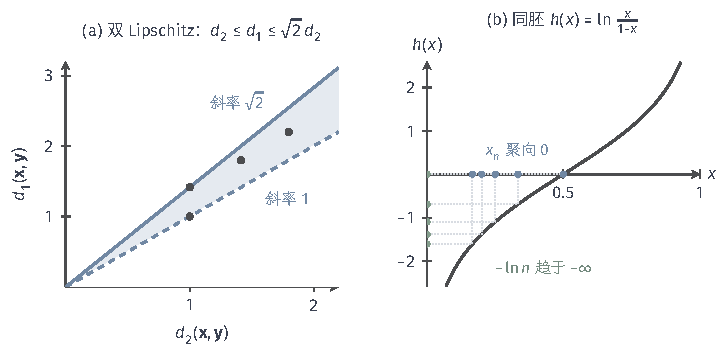
\includegraphics[width=123.261mm]{figures/02-abstract-mathematics/01-metric-and-measure/tikz/c1-bilipschitz-homeo/figure.pdf}
  \caption{双Lipschitz映射与同胚的区别。(a) 恒等映射$(\mathbb R^2,d_2)\to(\mathbb R^2,d_1)$：横轴为输入距离$d_2$，纵轴为输出距离$d_1$，所有点对都落在斜率$1$与$\sqrt2$两条直线之间的蓝色楔形中，输出误差与输入误差相差不超过常数倍。(b) logit同胚$h(x)=\ln(x/(1-x))$：横轴上的蓝点$x_n=1/(n+1)$（$n=1,\dots,5$）向$0$聚拢，构成柯西列，纵轴上的像$-\ln n$却越拉越远并趋于$-\infty$。}
  \label{fig:metric-bilipschitz-homeo}
\end{figure*}

这个例子同时说明，完备性不是只由开集决定的性质：$\mathbb R$上的通常距离$|s-t|$与$d'(s,t)=|\sigma(s)-\sigma(t)|$给出相同的开集（$\sigma:\mathbb R\to(0,1)$是同胚），但$(\mathbb R,|\cdot|)$完备，而在$d'$下点列$t_n=n$满足$d'(t_m,t_n)=|\sigma(m)-\sigma(n)|\to0$，是柯西列，却没有极限：若在$d'$下$t_n\to t$，则$\sigma(n)\to\sigma(t)<1$，与$\sigma(n)\to1$矛盾。讨论完备性、全有界性以及下一节的压缩条件时，必须指明所用的度量；只说“拓扑相同”不够。

\section{压缩映射与不动点}
\label{sec:metric-contraction}

章首的迭代$x^{(t+1)}=x^{(t)}/2+1$想求的是方程$x=x/2+1$的解。很多方程都可以写成$x=T(x)$的形式，再从一个初值出发反复应用$T$。本节把前面的工具用在同一个构造问题上：距离控制给出误差的几何衰减，柯西列与完备性给出极限的存在，连续性验证极限确实是解。然后讨论迭代应在何时停止，以及每步计算有误差时结论怎样修改。本节用带括号的上标$x^{(t)}$表示第$t$次迭代的结果。

\subsection{压缩映射定理}
\label{sec:metric-contraction-theorem}

满足$T(x^\star)=x^\star$的点$x^\star$称为$T$的\term{不动点}（fixed point）。迭代能否找到不动点，取决于$T$是否一致地拉近任意两点。

\begin{definition}[压缩映射]
\label{def:metric-contraction}
设$(X,d)$是度量空间，$T:X\to X$。若存在常数$0\leq q<1$，使所有$x,y\in X$都满足$d(T(x),T(y))\leq q\,d(x,y)$，就称$T$为\term{压缩映射}（contraction mapping），$q$称为压缩常数。
\end{definition}

压缩映射是Lipschitz常数小于$1$的自映射：它把$X$映回$X$自身，所以迭代可以无限进行下去；它对所有点对使用同一个$q$，所以每一步都至少把距离缩小到原来的$q$倍。

\begin{theorem}[压缩映射定理]
\label{thm:metric-contraction}
设$(X,d)$是非空完备度量空间，$T:X\to X$是压缩常数为$q$的压缩映射。则$T$有唯一的不动点$x^\star$，并且对任意初值$x^{(0)}\in X$，迭代$x^{(t+1)}=T(x^{(t)})$收敛到$x^\star$。
\end{theorem}

\begin{proof}
\emph{相邻差几何衰减。}由压缩条件，
\[
  d(x^{(t+1)},x^{(t)})=d\bigl(T(x^{(t)}),T(x^{(t-1)})\bigr)\leq q\,d(x^{(t)},x^{(t-1)}),
\]
反复使用得到$d(x^{(t+1)},x^{(t)})\leq q^t\,d(x^{(1)},x^{(0)})$。

\emph{迭代列是柯西列。}对$s>t$，沿中间各项用三角不等式，再对几何级数求和：
\begin{equation}
\label{eq:metric-contraction-tail}
  \begin{aligned}
    d(x^{(s)},x^{(t)})&\leq\sum_{k=t}^{s-1}d(x^{(k+1)},x^{(k)})
    \leq\sum_{k=t}^{s-1}q^k\,d(x^{(1)},x^{(0)})\\
    &\leq\frac{q^t}{1-q}\,d(x^{(1)},x^{(0)}).
  \end{aligned}
\end{equation}
因为$0\leq q<1$，右边在$t\to\infty$时趋于零，且与$s$无关，所以$(x^{(t)})$是柯西列。

\emph{极限存在且是不动点。}$X$完备，所以存在$x^\star\in X$使$x^{(t)}\to x^\star$。压缩映射是Lipschitz映射，因而连续，由序列判据$T(x^{(t)})\to T(x^\star)$。而$T(x^{(t)})=x^{(t+1)}\to x^\star$，由极限唯一，$T(x^\star)=x^\star$。

\emph{唯一性。}若$T(y^\star)=y^\star$，则$d(x^\star,y^\star)=d(T(x^\star),T(y^\star))\leq q\,d(x^\star,y^\star)$，即$(1-q)\,d(x^\star,y^\star)\leq0$。由$q<1$，$d(x^\star,y^\star)=0$，$x^\star=y^\star$。
\end{proof}

对$T(x)=x/2+1$，在$\mathbb R$上$|T(x)-T(y)|=|x-y|/2$，$q=1/2$，$\mathbb R$完备，所以有唯一不动点；解$x=x/2+1$得$x^\star=2$。从$x^{(0)}=0$出发，迭代依次为$0,\ 1,\ 1.5,\ 1.75,\ 1.875,\ 1.9375,\dots$，误差$|x^{(t)}-2|=2^{1-t}$每步减半。图~\ref{fig:metric-contraction}(a)用蛛网图画出了这个过程：在$y=T(x)$与$y=x$之间来回走折线，折线逐步收拢到两线的交点。

\paragraph{各条件的职责}
定理的四个条件各有作用，缺一不可。非空保证有初值可取。自映射保证每次迭代都留在$X$中。完备性提供极限：$T(x)=x/2$作为$(0,1)\to(0,1)$的映射满足$q=1/2$，迭代$x^{(t)}=2^{-t}x^{(0)}$是柯西列，但它在$\mathbb R$中的极限$0$不在$(0,1)$中，$T$在$(0,1)$上没有不动点。统一的$q<1$提供几何衰减：平移$T(x)=x+1$满足$|T(x)-T(y)|=|x-y|$，常数等于$1$，在完备的$\mathbb R$上却没有不动点。仅仅“相邻距离逐渐变小”也不够：$x^{(t)}=\sum_{k=1}^t1/k$的相邻差$1/(t+1)$趋于零，点列却趋于无穷，因为相邻差之和发散；压缩条件保证的是相邻差按几何级数衰减，其和有限。

\subsection{迭代误差与停止条件}
\label{sec:metric-contraction-error}

实际计算只能进行有限步，需要在不知道$x^\star$的情况下判断当前结果有多准确。证明中的几何尾和给出了答案。

\paragraph{先验与后验误差界}
在式~\eqref{eq:metric-contraction-tail}中令$s\to\infty$。由$d(\cdot,x^{(t)})$的连续性，左边趋于$d(x^\star,x^{(t)})$，于是得到\term{先验误差界}（a priori error bound）
\begin{equation}
\label{eq:metric-a-priori}
  d(x^{(t)},x^\star)\leq\frac{q^t}{1-q}\,d(x^{(1)},x^{(0)}).
\end{equation}
它只用第一步的位移，迭代开始前就能算出达到给定精度所需的步数。若把第$t-1$步看作新的初值，同一个估计给出$d(x^{(t)},x^\star)\leq\dfrac{q}{1-q}\,d(x^{(t)},x^{(t-1)})$，称为\term{后验误差界}（a posteriori error bound）
\begin{equation}
\label{eq:metric-a-posteriori}
  d(x^{(t)},x^\star)\leq\frac{q}{1-q}\,d(x^{(t)},x^{(t-1)}).
\end{equation}
它使用当前的相邻差，迭代过程中可以随时检查。

\begin{example}[按目标精度停止]
\label{ex:metric-contraction-stop}
对$T(x)=x/2+1$、$x^{(0)}=0$，有$q=1/2$、$d(x^{(1)},x^{(0)})=1$，先验界为$2^{1-t}$。要求误差不超过$10^{-3}$，需要$2^{t-1}\geq1000$；由$2^9=512<1000\leq1024=2^{10}$，取$t=11$，此时$x^{(11)}=1.9990234375$，误差$2^{-10}\approx0.000977$。后验界的系数$q/(1-q)=1$，例如$t=5$时$d(x^{(5)},x^{(4)})=1.9375-1.875=0.0625$，后验界为$0.0625$，而实际误差$|1.9375-2|=0.0625$。这个线性例子中两个误差界都恰好取等号。
\end{example}

\paragraph{收缩缓慢时的停止判断}
后验界中的系数$q/(1-q)$在$q$接近$1$时很大，小的相邻差可能对应大的误差。取$T(x)=0.99x+1$，它在$\mathbb R$上是$q=0.99$的压缩映射，不动点为$x^\star=100$。从$x^{(0)}=0$出发，$x^{(t)}=100(1-0.99^t)$，相邻差$d(x^{(t+1)},x^{(t)})=0.99^t$。当$t=459$时相邻差约为$0.00992$，首次小于$0.01$；而此时$x^{(460)}$的误差$100\cdot0.99^{460}\approx0.982$，几乎是相邻差的$99$倍，与后验界一致。若只凭“相邻两次变化小于$0.01$”就停止，结果会差将近$1$。先验界$100\cdot0.99^t\leq10^{-3}$要求$t\geq\ln(10^{-5})/\ln0.99\approx1145.5$，即约$1146$步，而$q=1/2$时只需$11$步。两个例子都满足定理的全部条件，定理保证收敛，却不保证收敛得快。

\subsection{带误差的压缩迭代}
\label{sec:metric-inexact-contraction}

实际计算中，$T(x^{(t)})$往往只能近似求出，例如受浮点舍入或内层迭代截断的影响。设精确映射$T$仍满足压缩条件，而实际得到的$x^{(t+1)}\in X$满足
\[
  d(x^{(t+1)},T(x^{(t)}))\leq\eta_t,
\]
其中$\eta_t\geq0$是第$t$步的执行误差。近似点必须仍在$X$中，否则压缩条件无从使用。

\paragraph{误差递推}
令$e_t=d(x^{(t)},x^\star)$。由三角不等式与$T(x^\star)=x^\star$，
\[
  e_{t+1}\leq d(x^{(t+1)},T(x^{(t)}))+d(T(x^{(t)}),T(x^\star))\leq\eta_t+q\,e_t.
\]
反复代入得到
\begin{equation}
\label{eq:metric-inexact-error}
  e_t\leq q^t e_0+\sum_{s=0}^{t-1}q^{t-1-s}\eta_s.
\end{equation}
第一项是初始误差的几何衰减，与精确迭代相同；第二项是各步新引入的误差，它们被后续步骤按$q$的幂次逐渐压缩，但不会消失。

\begin{theorem}[带误差的压缩迭代]
\label{thm:metric-inexact-contraction}
在上述设定下：(1) 若$\eta_t\leq\eta$对所有$t$成立，则$e_t\leq q^te_0+\eta/(1-q)$，从而$\limsup_{t\to\infty}e_t\leq\eta/(1-q)$；(2) 若$\eta_t\to0$，则$e_t\to0$，即$x^{(t)}\to x^\star$。
\end{theorem}

\begin{proof}
(1) 在式~\eqref{eq:metric-inexact-error}中把每个$\eta_s$放大为$\eta$，得到$\sum_{s=0}^{t-1}q^{t-1-s}\eta\leq\eta\sum_{k=0}^\infty q^k=\eta/(1-q)$。再令$t\to\infty$，$q^te_0\to0$。

(2) 设$\varepsilon>0$，取$S$使$s\geq S$时$\eta_s<\varepsilon$。对$t>S$，把和式分成$s<S$与$s\geq S$两段：
\[
  \sum_{s=0}^{t-1}q^{t-1-s}\eta_s
  \leq q^{t-S}\sum_{s=0}^{S-1}\eta_s+\varepsilon\sum_{k=0}^{\infty}q^k
  =q^{t-S}\sum_{s=0}^{S-1}\eta_s+\frac{\varepsilon}{1-q},
\]
其中第一段用了$s<S$时$q^{t-1-s}\leq q^{t-S}$。$S$固定后，第一项在$t\to\infty$时趋于零，所以$\limsup_te_t\leq\varepsilon/(1-q)$。$\varepsilon$任意，故$e_t\to0$。
\end{proof}

\begin{example}[固定执行误差]
\label{ex:metric-inexact-example}
对$T(x)=x/2+1$，设每步实际计算$x^{(t+1)}=T(x^{(t)})+0.1$，即$\eta_t=0.1$。从$x^{(0)}=0$出发，迭代依次为$0,\ 1.1,\ 1.65,\ 1.925,\ 2.0625,\ 2.13125,\dots$，收敛到$x/2+1.1=x$的解$2.2$，与精确不动点$2$相差$0.2$。定理~\ref{thm:metric-inexact-contraction}(1)给出的界$\eta/(1-q)=0.1/(1/2)=0.2$在这里恰好达到。图~\ref{fig:metric-contraction}(b)比较了精确迭代与带误差迭代的误差：前者每步减半，后者先下降，再停在$0.2$附近。
\end{example}

\begin{figure*}[!htbp]
  \centering
  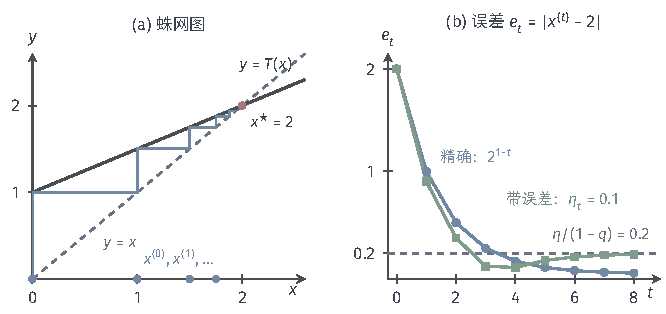
\includegraphics[width=112.691mm]{figures/02-abstract-mathematics/01-metric-and-measure/tikz/c1-contraction/figure.pdf}
  \caption{压缩迭代$T(x)=x/2+1$，初值$x^{(0)}=0$。(a) 蛛网图：从$x^{(0)}$出发竖直走到曲线$y=T(x)$，再水平走到对角线$y=x$，得到下一个迭代值；折线收拢到交点$x^\star=2$。(b) 误差$e_t=|x^{(t)}-2|$：蓝色为精确迭代，$e_t=2^{1-t}$；绿色为每步加入执行误差$0.1$的迭代，误差先下降，越过精确解后趋向$0.2$；灰色虚线是误差上界$\eta/(1-q)=0.2$。}
  \label{fig:metric-contraction}
\end{figure*}

\paragraph{带误差时的停止判断}
执行误差也改变停止判断。对任意$x\in X$，$d(x,x^\star)\leq d(x,T(x))+d(T(x),T(x^\star))\leq d(x,T(x))+q\,d(x,x^\star)$，所以$d(x,x^\star)\leq d(x,T(x))/(1-q)$。取$x=x^{(t)}$，并用$d(x^{(t)},T(x^{(t)}))\leq d(x^{(t)},x^{(t+1)})+\eta_t$，得到
\[
  e_t\leq\frac{d(x^{(t+1)},x^{(t)})+\eta_t}{1-q}.
\]
可观测的相邻差必须连同本步执行误差一起判断：在上例中，迭代停在$2.2$附近时相邻差趋于零，但$\eta_t=0.1$使右边始终不小于$0.2$，正确地提示结果并没有比$0.2$更准。本节只保留这一通用机制；线性方程组的迭代解法和最优化中的迭代算法，会在相应部分利用具体结构给出压缩常数。

\section{本章小结}
\label{sec:metric-summary}

本章从实数的绝对值、向量的范数、二进制串的Hamming距离和图的最短路距离中提炼出度量的三条要求，并说明度量是空间结构的一部分：同一集合换一个度量，球的形状、哪些点列收敛、是否可分都可能改变。距离依次提供了三层语言。开球给出邻近结构，由它定义开集、闭集、闭包与稠密；点列收敛把邻近变成可以逐项检查的误差，闭集的序列判据把两者连起来；连续映射研究误差在两个空间之间的传递，一致连续与Lipschitz条件分别要求统一的容差与统一的放大倍数。

几个“有限性”与“存在性”条件分别控制不同的对象。有界控制集合的总体范围；可分要求一套可数代表服务所有精度；全有界要求每个精度只需有限个代表；完备要求柯西列在空间内有极限；紧致要求每个给定的开覆盖都有有限子覆盖。在度量空间中，紧致等价于序列紧致，也等价于完备且全有界；只有在$\mathbb R^d$这样的有限维欧氏空间中，才可以简化为闭且有界。紧致定义域使连续函数取得最值、使最近点存在、使连续升级为一致连续，但不提供Lipschitz常数。比较两个空间时，双Lipschitz映射保留柯西列、完备性和全有界性，同胚只保留开集与收敛；logit映射表明，完备性不是由开集单独决定的。

压缩映射定理把这些结论串成一条完整的论证：统一的压缩常数使相邻差几何衰减，几何尾和使迭代列成为柯西列，完备性给出极限，连续性验证极限满足$T(x^\star)=x^\star$，压缩条件再给出唯一性。同一条尾和估计给出先验与后验误差界，带误差的版本说明执行误差会留下$\eta/(1-q)$量级的偏差。各个反例提醒我们：只观察到相邻项越来越近，或在局部看到误差缩小，都不足以断定极限存在或结果准确；每个结论都需要它的全部条件。

下一章转向另一个问题：怎样测量一个集合的大小。度量空间的开集将生成Borel集合族，为测量提供可用的集合；但距离本身并不决定集合的测度，同一个度量空间上可以有许多不同的测度。

